\documentclass[a4paper, 12pt]{article}
% load fonts first
% https://docs.google.com/spreadsheets/d/1vpwFNgv8czllJUqdmP3EGDLYPrRMSalF66uRko_lkfM/edit?gid=2134328593
% load encodings later
\usepackage[T1]{fontenc}
\usepackage[utf8]{inputenc}

% finally load babel
\usepackage{csquotes}
\usepackage[english,spanish]{babel}
\decimalpoint
%\selectlanguage{spanish}

% % % % % % % DEFINICIONES E IDENTIFICACIÓN

\newcommand\mInstituto{Universidad Nacional de San Agustín de Arequipa}
\newcommand\mFacultad{Facultad de Ingeniería de Producción y Servicios}
\newcommand\mEscuela{Escuela Profesional de Ingeniería de Sistemas}
\newcommand\mCurso{Análisis y Diseño de Algoritmos}
\newcommand\mNumeroP{P2}
\newcommand\mTituloP{Programación Dinámica}
\newcommand\mFechaE{14 de Nov.}
\newcommand\mEstudiante{20230464, SEQUEIROS CONDORI LUIS GUSTAVO} % < < < Coloque sus datos aquí ! ! !

% % % % % % % INICIO DE PAQUETES Y UTILITARIOS [ * [ no editar hasta la línea 150 ] * ]
\usepackage[paper=a4paper,twoside=false,top=15mm,bottom=2cm,inner=2cm,outer=2cm,headsep=2mm,headheight=15pt,footskip=11pt]{geometry}

% \usepackage{amsmath,mathtools,amssymb}% amssymb calls amsfonts
\usepackage[bigdelims,varg]{newtxmath}
\usepackage{newtxtext} % options will be as passed from newtx

\usepackage{setspace}%provides:setstretch,singlespacing,onehalfspacing,doublespacing
\usepackage{pgfplots}
\pgfplotsset{compat=1.18}
\usepackage{tikz}
\usetikzlibrary{arrows,arrows.meta,positioning,tikzmark,shapes}
% \usetikzlibrary{arrows.meta,positioning,tikzmark,decorations.pathmorphing,decorations.pathreplacing,patterns,fit,backgrounds,calc,shapes,shapes.multipart,shapes.misc}
\usepackage{graphicx}
\graphicspath{{./}{imgs/}}
\usepackage{booktabs,multirow,rotating,array,color,colortbl}%for better tables
\newcolumntype{L}[1]{>{\raggedright\let\newline\\\arraybackslash\hspace{0pt}}m{#1}}
\newcolumntype{R}[1]{>{\raggedleft\let\newline\\\arraybackslash\hspace{0pt}}m{#1}}
\newcolumntype{C}[1]{>{\centering\let\newline\\\arraybackslash\hspace{0pt}}m{#1}}
\newcolumntype{J}[1]{>{\let\newline\\\arraybackslash\hspace{0pt}}m{#1}}
\newcolumntype{j}[1]{>{\let\newline\\\arraybackslash\hspace{0pt}}p{#1}}
\usepackage{hyperref}
\definecolor{spot}{rgb}{0,0,0.5}
\hypersetup{citecolor=spot,urlcolor=spot,linkcolor=spot,colorlinks,plainpages=false}
\usepackage{enumitem}
\setlist{nosep,noitemsep}

% \usepackage[ruled]{algorithm}
\usepackage[noend]{algpseudocode}
\algrenewcommand\algorithmicindent{1em}
% \usepackage[noEnd=true,commentColor=structure]{algpseudocodex} % TODO: try, looks better
\algnewcommand\mInput{\item[\textbf{Input:}] }
\algnewcommand\mOutput{\item[\textbf{Output:}] }
\algrenewcommand\Return{\State\algorithmicreturn{} }
% \algrenewcommand\algorithmicindent{1.0em}
% \algrenewcommand\alglinenumber[1]{\footnotesize\makebox[5mm][r]{#1:}}%

\usepackage[explicit]{titlesec}
\titlespacing*{\section}{0pt}{8pt plus 12pt minus 4pt}{4pt plus 6pt minus 4pt}
\titlespacing*{\subsection}{0pt}{6pt plus 12pt minus 4pt}{3pt plus 6pt minus 2pt}
\titlespacing*{\subsubsection}{0pt}{6pt plus 12pt minus 4pt}{3pt plus 6pt minus 2pt}

\usepackage[backend=biber,style=apa,natbib=true,sorting=nyt,citereset=none,
maxbibnames=8, minbibnames=1, maxcitenames=2]{biblatex}
\DeclareLanguageMapping{spanish}{spanish-apa}
\DefineBibliographyStrings{spanish}{andothers={et~al\adddot}}
\defbibheading{bibliography}[Referencias Bibliográficas]{\section{#1} \addcontentsline{toc}{section}{#1}}
\addbibresource{biblio.bib}

\usepackage{fancyhdr}
\pagestyle{fancy}
\fancypagestyle{plain}{\fancyhf{}\renewcommand{\headrulewidth}{0pt}
\fancyfoot[C]{\scriptsize\emph{Página \thepage\ de \pageref{pg:lastpage}}}}
\fancyhf{}
\renewcommand{\headrulewidth}{0.5pt}
\setlength{\headsep}{7mm}
\fancyhead[L]{\mCurso}
\fancyhead[R]{Práctica de \mTituloP}
\fancyfoot[C]{\scriptsize\emph{Página \thepage\ de \pageref{pg:lastpage}}}
\AtEndDocument{\label{pg:lastpage}}

\usepackage{listings}
\lstloadlanguages{C++}%default:{[ISO]C++}

\lstdefinestyle{mCpp}{language=C++,tabsize=2,aboveskip=3pt,belowskip=1pt,
columns=fixed,basewidth=4pt,fontadjust=true,breakatwhitespace=true,
prebreak=\raisebox{0ex}[0ex][0ex]{\ensuremath{\hookleftarrow}},inputencoding=utf8,
basicstyle=\scriptsize\ttfamily,keywordstyle=\color{blue}\bfseries,
identifierstyle=,commentstyle=\color[rgb]{.5,.5,.5},stringstyle=\color[rgb]{0.627,0.126,0.941},
numbers=left,numbersep=3pt,numberstyle=\color{blue},
frame=none,showtabs=false,showspaces=false,showstringspaces=true,
}

\lstset{style=mCpp}

\makeatletter
\renewcommand\maketitle{%
\setcounter{section}{0}\setcounter{page}{1}%
\newpage\null\vskip -2cm%
\begingroup\thispagestyle{plain}\centering
\def\mWd{165mm}{\setlength{\tabcolsep}{0pt}
\begin{tabular}{|c|c|c|}
\hline\makebox[2cm]{\begin{tikzpicture}[anchor=center,baseline,scale=0.06]
\definecolor{uRed}{RGB}{101,29,50}
\fill[rotate=50,fill=black!25]circle(12 and 8);
\fill[fill=uRed](-12,-7)--(-2,-3)--(-12,1)--cycle;
\fill[fill=uRed](12,7)--(2,3)--(12,-1)--cycle;
\end{tikzpicture}}&\makebox[129mm]{\tikz[anchor=center,baseline]
\node[text width=12cm,text centered]{\MakeUppercase{\mInstituto\\\mFacultad\\\mEscuela}};}
&\makebox[2cm]{\begin{tikzpicture}[anchor=center,baseline,black!60,shift={(0pt,7.4pt)}]
\definecolor{cABET}{RGB}{243,108,56}
\draw[cABET,line width=3.55pt] circle(11.85pt);
\fill[line width=0.05pt] (-0.74,-1)--(-0.62,-0.67)--(-0.525,-0.67)--
(-0.405,-1)--(-0.5,-1)--(-0.52,-0.94)--(-0.62,-0.94)--(-0.64,-1)--cycle
(-0.54,-0.87)--(-0.57,-0.77)--(-0.6,-0.87)--cycle;
\fill[line width=0.05pt] (-0.3,-1)--(-0.3,-0.67)--
(-0.11,-0.67)to[out=0,in=35,distance=2.3pt](-0.06,-0.82)
to[out=-30,in=0,distance=2.6pt](-0.11,-1)--cycle
(-0.21,-0.925)--(-0.135,-0.925)to[out=0,in=0,distance=0.8pt]
(-0.135,-0.865)--(-0.21,-0.865)--cycle
(-0.21,-0.79)--(-0.135,-0.79)to[out=0,in=0,distance=0.7pt]
(-0.135,-0.745)--(-0.21,-0.745)--cycle;
\fill[line width=0.05pt] (0.1,-1)--(0.1,-0.67)--(0.348,-0.67)--
(0.348,-0.75)--(0.19,-0.75)--(0.19,-0.79)--(0.285,-0.79)--(0.285,-0.867)--
(0.19,-0.867)--(0.19,-0.925)--(0.348,-0.925)--(0.348,-1)--cycle;
\fill[line width=0.05pt] (0.56,-1)--(0.56,-0.75)--(0.464,-0.75)--
(0.464,-0.67)--(0.736,-0.67)--(0.736,-0.75)--
(0.645,-0.75)--(0.645,-1)--(0.348,-1)--cycle;
\end{tikzpicture}}\\\hline
\end{tabular}\\[4mm]}
\textbf{\Large INFORME DE LABORATORIO}\\[4mm]
{\small\begin{tabular}{|>{\bf}L{29mm}|L{23mm}|>{\bf}L{29mm}|L{17mm}|>{\bf}L{29mm}|L{16mm}|}
\hline\multicolumn{6}{|m{\mWd}|}{\vspace{3mm}\centering\large
\color{white}\cellcolor{red!50!black}INFORMACIÓN BÁSICA\vspace{2mm}}\\\hline
ASIGNATURA:&\multicolumn{5}{|l|}{\MakeUppercase\mCurso} \\\hline
TÍTULO DE LA \linebreak PRÁCTICA:&\multicolumn{5}{|l|}{\MakeUppercase\mTituloP} \\\hline
NÚMERO DE PRÁCTICA:&\mNumeroP&AÑO LECTIVO:&2024&SEMESTRE:&PAR
\\\hline\multicolumn{6}{|L{\mWd}|}{{\bf ESTUDIANTES:}\newline\mEstudiante}\\\hline
\multicolumn{6}{|l|}{{\bf DOCENTES:} Marcela Quispe Cruz, Manuel Loaiza, Alexander J. Benavides}\\\hline
\end{tabular}\\[4mm]
\large\begin{tabular}{|L{\mWd}|}\hline\multicolumn{1}{|m{\mWd}|}{\vspace{3mm}\centering
\color{white}\cellcolor{red!50!black}RESULTADOS Y PRUEBAS\vspace{2mm}}\\\hline
El informe se presenta con un formato de artículo.\\Revise la sección de \emph{Resultados Experimentales}.
\\\hline\multicolumn{1}{l}{}\\\hline\multicolumn{1}{|m{\mWd}|}{\vspace{3mm}\centering
\color{white}\cellcolor{red!50!black}CONCLUSIONES\vspace{2mm}}\\\hline
El informe se presenta con un formato de artículo.\\Revise la sección de \emph{Conclusiones}.
\\\hline\multicolumn{1}{l}{}\\\hline\multicolumn{1}{|m{\mWd}|}{\vspace{3mm}\centering
\color{white}\cellcolor{red!50!black}METODOLOGÍA DE TRABAJO\vspace{2mm}}\\\hline
El informe se presenta con un formato de artículo.\\Revise la sección de \emph{Diseño Experimental}.
\\\hline\multicolumn{1}{l}{}\\\hline\multicolumn{1}{|m{\mWd}|}{\vspace{3mm}\centering
\color{white}\cellcolor{red!50!black}REFERENCIAS Y BIBLIOGRAFÍA\vspace{2mm}}\\\hline
El informe se presenta con un formato de artículo.\\Revise la sección de \emph{Referencias Bibliográficas}.
\\\hline\end{tabular}\newpage}\endgroup}
\makeatother

\setlength{\textfloatsep}{14pt plus 10pt minus 10pt}%20+2-4
\setlength{\floatsep}{12pt plus 8pt minus 8pt}%12+2-4
\setlength{\intextsep}{10pt plus 6pt minus 4pt}%14+4-4
\setlength{\abovecaptionskip}{2pt plus 2pt minus 2pt}%
\setlength{\belowcaptionskip}{-1pt plus 1pt minus 1pt}%
\setlength{\parskip}{8pt plus 6pt minus 4pt}%
\setlength{\parindent}{0pt}

\def\bigO{\mathcal{O}}
\def\enmax{\mathrm{max}}
\usepackage{lipsum}


% % % % % % % FIN DE PAQUETES Y UTILITARIOS [ * [ no editar desde la línea 20 ] * ]


\singlespacing
\begin{document}
\maketitle

{\centering\Large Programación Dinámica $-$ Ejemplos de Aplicación\par}
% Ponga su identificación SOLAMENTE en la carátula del informe.
% El artículo se calificará de manera ciega.

\section*{\emph{Resumen}}
Este artículo explora la aplicación del método SRTBOT y la programación dinámica en la resolución de problemas de programación competitiva. A partir de una selección aleatoria de problemas, se empleó una metodología de diseño que permite descomponer cada problema en subproblemas. Luego, se aplicó memoización para optimizar el uso de recursos y mejorar la eficiencia de las soluciones. La implementación inicial en Python facilitó la validación de la lógica y la depuración de errores, mientras que la versión final en C++ optimizó el rendimiento en términos de tiempo de ejecución.

El objetivo de este trabajo fue fortalecer el conocimiento en programación dinámica y familiarizarse con el uso del método SRTBOT. Entre los principales logros se encuentran el desarrollo de soluciones eficientes y el aprendizaje de técnicas avanzadas de modelado y análisis algorítmico. Las dificultades encontradas incluyeron la correcta identificación de casos base y la optimización de la estructura recursiva en problemas con restricciones complejas.

Este artículo se organiza de la siguiente forma: se presenta la teoría y el contexto de las técnicas utilizadas, el diseño experimental para la selección de problemas, la implementación de las soluciones y, finalmente, las conclusiones donde se destacan los logros y las áreas de mejora.

\section{Introducción}
\label{sc:intro}
% La introducción debe presentar la información necesaria para entender el resto del artículo.
% Describe el contexto del problema a ser resuelto y su importancia.
% Explica los principales aportes y los objetivos alcanzados con el trabajo.
% Una buena introducción genera en el lector un mayor interés para leer el resto del artículo.
% Es más fácil escribir la introducción
% luego de completar el resto del artículo.

% Esta sección termina con una breve explicación de lo que muestran el resto del artículo.
Una forma de entrenar la resolución de problemas y la construcción de algoritmos es mediante la resolución de problemas de programación competitiva. Este artículo se enfoca en el uso de técnicas avanzadas, como el método SRTBOT y la programación dinámica, para abordar problemas complejos de manera estructurada y eficiente. Estas técnicas permiten descomponer problemas en subproblemas más pequeños y reutilizar soluciones previas. De esta manera, se optimizan los recursos computacionales necesarios para la ejecución.

El objetivo principal de este trabajo es reforzar los conocimientos en programación dinámica y aplicar el método SRTBOT para la resolución de problemas. A través de esta experiencia, se pretende consolidar habilidades en el diseño de algoritmos recursivos optimizados. Los logros alcanzados incluyen el análisis sistemático de cada problema y la implementación de soluciones eficientes C++.

El resto del artículo está organizado de la siguiente manera. La \autoref{sc:teoria} describe los fundamentos teóricos de las técnicas utilizadas. La \autoref{sc:DisExp} presenta el diseño experimental y el proceso de selección de problemas. La \autoref{sc:Experim} muestra los resultados obtenidos en la implementación de las soluciones. Finalmente, la \autoref{sc:Concl} expresa las conclusiones del trabajo, resaltando los logros alcanzados y las dificultades encontradas.

\section{Marco Teórico Conceptual}
\label{sc:teoria}

% Esta sección presenta formalmente los conceptos teóricos necesarios
% para entender cabalmente el problema y los métodos de solución.
% El marco conceptual esta conformado por conceptos, definiciones y métodos
% que forman parte del conocimiento general del problema
% ampliamente difundido en libros y artículos.
% Por ejemplo, si estudiamos programación dinámica, debe introducir los conceptos necesarios.

Programación dinámica fue propuesta por \citet{bellman1952theory}.
Esta es una técnica que busca la resolución de problemas que pueden ser divididos en subproblemas superpuestos, cada uno de ellos tiene una solución independiente y considerada óptima. Por ello, estas subsoluciones pueden ser almacenadas y recordadas cuando sea necesario; de esta manera se mejora la eficiencia de la solución. Asimismo, la solución del problema general viene dada por la unión de las soluciones óptimas de los subproblemas.

El nemotécnico SRTBOT propuesto por \citet{demaine2021} ayuda en el diseño de  algoritmos recursivos para resolver un problema. A continuación, se explican los seis conceptos de SRTBOT.

\textbf{Subproblemas} El primer paso consiste en dividir el problema original en subproblemas. Para esto es necesario definir etapas y estados, así como las transiciones entre ellos. Se deben considerar las precondiciones y postcondiciones del problema. De este modo, se puede modelar la signatura de una función que aplique programación dinámica.

\textbf{Relaciones Recursivas} En este paso se deben relacionar, unir o combinar las subsoluciones de manera que se obtenga una solución óptima dependiendo del tipo de problema. En esta etapa se modela la implicación matemática de la función.

\textbf{Topología} Dibujar la topología ayuda a comprender cómo se relacionan las etapas, estados y sus transiciones. Asimismo, ayuda a visualizar el flujo del problema. De esta forma, se corrobora que el problema va a tener una solución finita.

\textbf{Bases} Aquí se formalizan los casos base. Un caso base se define como la situación o estado en el que el problema tiene una solución ya conocida y simple. Por lo tanto, no es necesario calcularla con subsoluciones.

\textbf{Original} Ahora se debe resolver el problema original; es decir,
con la información de los cuatro puntos anteriores se diseña el algoritmo recursivo en pseudocódigo. Agregar {\bf memoización} ayudará a mejorar la eficiencia de la solución gracias al almacenamiento de soluciones a subproblemas superpuestos.

\textbf{Tiempo} Finalmente se debe analizar el tiempo de ejecución de la solución para confirmar su eficiencia. En caso no sea eficiente, es recomendable analizar nuevamente la solución y optimizarla o utilizar otro enfoque diferente de programación dinámica.

\section{Diseño Experimental}
\label{sc:DisExp}

A continuación, se describen los pasos que se siguieron en esta investigación para seleccionar y dar solución a los problemas escogidos.

% En nuestro caso el estudiante deberá explicar en esta sección el proceso seguido para seleccionar y resolver los problemas propuestos. A continuación estan descritos los objetivos y las actividades de este trabajo. El estudiante \textbf{\emph{deberá cambiarlos}} a tiempo pasado, detallando más los pasos, indicando los logros alcanzados y las dificultades encontradas (si hubieran).


\subsection{Objetivos}

Los objetivos de este trabajo son:
\begin{itemize}
  \item
        Reforzar los conocimientos del método de programación dinámica.
  \item
        Aplicar el método de programación dinámica para resolver algunos problemas propuestos.
\end{itemize}

\subsection{Actividades}

El estudiante deberá realizar las siguientes acciones.
\begin{enumerate}
  \item
        Se creó un usuario en \href{http://vjudge.net}{http://vjudge.net} dientificado como \textbf{\href{http://vjudge.net/user/gustadev}{gustadev}}. El registro permitió acceder a una variedad de problemas de programación competitiva en un entorno unificado. Asimismo, facilitó el seguimiento de los resultados y la evaluación del progreso.
  \item
        Se seleccionaron aleatoriamente tres problemas de la lista disponible en
        \url{http://bit.ly/3UxdCVL}. Al cargar la hoja de cálculo con la lista de problemas, se combinó su orden utilizando una función de mezcla aleatoria para asegurar una distribución imparcial. A partir de esta lista mezclada, se generaron tres números aleatorios utilizando el generador de números aleatorios de Google, lo que permitió determinar las posiciones de los problemas seleccionados.
  \item
        Se diseñaron soluciones para cada problema utilizando la técnica SRTBOT. Esta técnica facilitó el modelado de las soluciones gracias al análisis estructurado del problema antes de la implementación. Durante este proceso, se encontraron algunas dificultades en la identificación de subproblemas y en la optimización del enfoque recursivo. Para este último, en los tres problemas se tuvo dificultades, ya que no se identificaron condiciones de quiebre al comienzo el diseño. Esto se traducía en cálculos de subsoluciones innecesarios.
  \item
        Se elaboraron dos versiones del pseudocódigo recursivo para cada problema: una versión inicial sin memoización y una versión optimizada con memoización. Esto permitió comparar el impacto de la optimización en términos de eficiencia y comprender mejor los beneficios del almacenamiento de resultados previos.
  \item
        Se implementaron las soluciones en \texttt{C++} siguiendo el modelo SRTBOT. Esta implementación en C++ se realizó tras verificar la funcionalidad en Python. Se hicieron notorias mejoras significativas en términos de tiempo de ejecución y aprovechamiento de memoria.
  \item
        Se generó un PDF de cada solución aceptada en la plataforma \href{http://vjudge.net}{http://vjudge.net} y se anexó al final del artículo como evidencia de la correcta resolución de los problemas. Esto sirvió para demostrar la efectividad de las soluciones y el cumplimiento de los objetivos del trabajo.
\end{enumerate}

\section{Resultados}
\label{sc:Experim}

En esta sección se muestra el proceso de resolución para cada uno de los problemas escogidos.

\subsection{Problema 10074 -- Take the Land}

\textbf{Subproblema:}
Encuentre $A(x, y, k, z)$ para las coordenadas de matriz $0\leq x < N$, $0\leq y < M$. Asimismo, para la base del mayor rectángulo $k$ y su altura permitida $z$, se cumple: $0 < k \leq x$, $0 < z \leq y$ si se trabaja horizontalmente y $0 < k \leq y$, $0 < z \leq x$ si es verticalmente. Para hallar la altura $z$ que cumple con las condiciones de un rectángulo $z = Z(x, y)$, donde la altura $Z$ se halla dependiendo la dirección: horizontal o vertical.

\textbf{Relaciones Recursivas: }\\[-3mm]
$$A(x,y,k,z)=\begin{cases}
    A(x+1,y,1,Z(x,y)),                  & Horizontal \land z = 0 \\
    A(x,y+1,1,Z(x,y)),                  & Vertical \land z = 0   \\
    \max(z*k,A(x+1,y,k+1,min(Z(x,y)))), & Horizontal \land z > 0 \\
    \max(z*k,A(x,y+1,k+1,min(Z(x,y)))), & Vertical \land z > 0
  \end{cases}$$
$$Z(x,y,k,z)=\begin{cases}
    M_{x,y} + Z(x+1,y), & Horizontal \\
    M_{x,y} + Z(x,y+1), & Vertical   \\
  \end{cases}$$

\textbf{Topología: }\\[-5mm]
\strut\hfill
\begin{tikzpicture}[inner sep=0pt,yscale=0.4]
  \tikzstyle{v}=[ellipse,thick,draw,minimum width=24mm,minimum height=6mm]\footnotesize
  \node[v](xyz)at(0,1){$x,y,z$};
  \node[v](x1yzmin)at(4,2){$x+1,y,z_{min}$};
  \node[v](xy1zmin)at(4,0){$x,y+1,z_{min}$};
  \node[v](n1yzmin)at(9.5,3){$N+1,y,z_{min}$};
  \node[v](ym1zmin)at(9.5,0){$x,M+1,z_{min}$};
  \foreach\i in{0,1,2,3}{\node(e\i)at(7.4,\i){...};}
  \tikzstyle{e}=[-Stealth,draw=black,very thick]
  \foreach\o/\d in{xyz/x1yzmin,xyz/xy1zmin,x1yzmin/e3,x1yzmin/e2,xy1zmin/e1,xy1zmin/e0}{\draw[e](\o.east)--(\d.west);}
\end{tikzpicture}\hfill\strut\par

\textbf{Básico:} $A(x,y,k,z) = 0$,\ $Z(x,y) = 0$ si $x \geq N \lor y \geq M$

\textbf{Original:}\\
\begin{minipage}[t]{78mm}
  \hrule{\bf Algorithm} A$(x,y,k,z,s)$\hfill// sin memoización\hrule
  \begin{algorithmic}[1]
    \mInput posición $x$, posición $y$, orientación $s$, valor $k$, mínimo de ceros $z$
    \mOutput área máxima
    \If{$y \geq M$ {\bf or} $x \geq N$}
    \Return $0$
    \EndIf
    \State $zc \gets \text{Z}(x, y, \neg s)$
    \State $minZ \gets$ \textbf{if} $z \neq 0$ \textbf{then} $\min(z, zc)$ \textbf{else} $zc$
    \State $maxA \gets 0$
    \State $vx \gets$ \textbf{if} $s$ es horizontal \textbf{then} $x + 1$ \textbf{else} $x$
    \State $vy \gets$ \textbf{if} $s$ es horizontal \textbf{then} $y$ \textbf{else} $y+1$
    \If{$minZ = 0$}
    \State $maxA \gets \text{A}(vx, vy, s, 1, minZ)$
    \Else
    \State $maxA \gets \max(minZ \cdot k,$ \\
      \hfill $\text{A}(vx, vy, s, k + 1, minZ))$
    \EndIf
    \Return $maxA$
  \end{algorithmic}
\end{minipage}\hfill
\begin{minipage}[t]{78mm}
  \hrule{\bf Algorithm} AM$(x,y,k,z,s)$\hfill// con memoización\hrule
  \begin{algorithmic}[1]
    \mInput posición $x$, posición $y$, orientación $s$, valor $k$, mínimo de ceros $z$
    \mOutput área máxima
    \If{$y \geq M$ {\bf or} $x \geq N$}
    \Return $0$
    \EndIf
    \State Inicializar $MZ$, memoria para $Z$
    \State $zc \gets \text{ZM}(x, y, \neg s)$
    \State $minZ \gets$ \textbf{if} $z \neq 0$ \textbf{then} $\min(z, zc)$ \textbf{else} $zc$
    \If{$M[x,y,s,minZ]\ is \ defined$}
    \Return $M[x,y,s,minZ]$
    \EndIf
    \State $maxA \gets 0$
    \State $vx \gets$ \textbf{if} $s$ es horizontal \textbf{then} $x + 1$ \textbf{else} $x$
    \State $vy \gets$ \textbf{if} $s$ es horizontal \textbf{then} $y$ \textbf{else} $y+1$
    \If{$minZ = 0$}
    \State $maxA \gets \text{AM}(vx, vy, s, 1, minZ)$
    \Else
    \State $maxA \gets \max(minZ \cdot k,$ \\
      \hfill $\text{AM}(vx, vy, s, k + 1, minZ))$
    \EndIf
    \State $M[x,y,s,minZ] \gets maxA$
    \Return $maxA$
  \end{algorithmic}

\end{minipage}\hfill\\[6mm]
\begin{minipage}[t]{78mm}
  \hrule{\bf Algorithm} Z$(x,y,s)$\hfill// sin memoización\hrule
  \begin{algorithmic}[1]
    \mInput posición $x$, posición $y$, orientación $s$
    \mOutput número de ceros consecutivos
    \If{$y \geq M$ {\bf or} $x \geq N$}
    \Return $0$
    \EndIf
    \State $r \gets 0$
    \If{$s$ es horizontal}
    \State $r \gets 1 + \text{Z}(x + 1, y, s, m)$
    \Else
    \State $r \gets 1 + \text{Z}(x, y + 1, s, m)$
    \EndIf
    \Return $r$
  \end{algorithmic}
\end{minipage}\hfill
\begin{minipage}[t]{78mm}
  \hrule{\bf Algorithm} ZM$(x,y,s)$\hfill// con memoización\hrule
  \begin{algorithmic}[1]
    \mInput posición $x$, posición $y$, orientación $s$
    \mOutput número de ceros consecutivos
    \If{$y \geq M$ {\bf or} $x \geq N$}
    \Return $0$
    \EndIf
    \If{$MZ[x,y,s]$}
    \Return $MZ[x,y,s]$
    \EndIf
    \State $r \gets 0$
    \If{$s$ es horizontal}
    \State $r \gets 1 + \text{ZM}(x + 1, y, s, m)$
    \Else
    \State $r \gets 1 + \text{ZM}(x, y + 1, s, m)$
    \EndIf
    \State $MZ[x,y,s] \gets r$
    \Return $r$
  \end{algorithmic}


\end{minipage}\hfill

\textbf{Tiempo:} AM$(x,y,k,z)\in \bigO(x*y)$, ZM$(x,y)\in \bigO(x,\ y)$

\textbf{Código:}\\

\strut\hspace{1cm}
\begin{minipage}[t]{7cm}
  \hrule\begin{lstlisting}
#include <iostream>
#include <vector>
#include <unordered_map>
#include <tuple>
#include <algorithm>

using namespace std;

struct MemoKey
{
  int x, y, minZ;
  bool s;
  bool operator==(const MemoKey &o) const
  {
    return tie(x, y, s) == tie(o.x, o.y, o.s);
  }
};

struct MemoKeyHash
{
  size_t operator()(const MemoKey &key) const
  {
    return hash<int>()(key.x)^hash<int>()(key.y)
    ^ hash<int>()(key.minZ)^hash<bool>()(key.s);
  }
};

int zeros(int x, int y, bool s,
const vector<vector<int>> &m,
unordered_map<MemoKey, int, MemoKeyHash> &mZ)
{
  if (y >= m.size() || x >= m[y].size())
    return 0;
  if (m[y][x] == 1)
    return 0;

  MemoKey key = {x, y, s};
  if (mZ.find(key) != mZ.end())
  {
    return mZ[key];
  }

  int result;
  if (s)
  {
    result = 1 + zeros(x + 1, y, s, m, mZ);
  }
  else
  {
    result = 1 + zeros(x, y + 1, s, m, mZ);
  }
  mZ[key] = result;
  return result;
}

int maxArea(int x, int y, bool s,
int k, int minZeros,
const vector<vector<int>> &m,
unordered_map<MemoKey, int, MemoKeyHash> &memo)
{
  if (y >= m.size() || x >= m[y].size())
    return 0;
  unordered_map<MemoKey, int, MemoKeyHash> mZ;
  int zerosC = zeros(x, y, !s, m, mZ);
  int minZ = (minZeros != 0)
  ? min(minZeros, zerosC) : zerosC;
  MemoKey key = {x, y, minZ, s};
  if (memo.find(key) != memo.end())
  {
    return memo[key];
  }
  int maxA = 0;
  if (minZ == 0)
\end{lstlisting}\hrule
\end{minipage}
\hfill
\begin{minipage}[t]{7cm}
  \hrule\begin{lstlisting}[firstnumber=74]
  {
    maxA = maxArea((s ? x + 1 : x),
    (s ? y : y + 1), s, 1, minZ, m, memo);
  }
  else
  {
    maxA = max(minZ * k, maxArea((s ? x + 1 : x),
    (s ? y : y + 1), s, k + 1, minZ, m, memo));
  }
  memo[key] = maxA;
  return maxA;
}

int max_land(int x, int y, bool s,
const vector<vector<int>> &m)
{
  int r = 0;
  unordered_map<MemoKey, int, MemoKeyHash> memo;

  if (s && x >= 0 && y >= 0)
  {
    for (int i = x; i < m[y].size(); ++i)
    {
      r = max(r,maxArea(i, y, s, 1, 0, m, memo));
    }
    if (x == 0)
    {
      r = max(r, max_land(x, y - 1, s, m));
    }
    else
    {
      r = max(r, max_land(x - 1, y, !s, m));
    }
  }
  else if (!s && y >= 0 && x >= 0)
  {
    for (int i = y; i < m.size(); ++i)
    {
      r = max(r,maxArea(x, i, s, 1, 0, m, memo));
    }
    if (y == 0)
    {
      r = max(r, max_land(x - 1, y, s, m));
    }
    else
    {
      r = max(r, max_land(x, y - 1, !s, m));
    }
  }
  return r;
}
int main()
{
  int m, n;
  cin >> m >> n;
  while (m != 0 || n != 0)
  {
    vector<vector<int>> grid(m, vector<int>(n));

    for (int i = 0; i < m; ++i)
    {
      for (int j = 0; j < n; ++j)
      {
        cin >> grid[i][j];
      }
    }

    cout <<
    max_land(n - 1, m - 1, true, grid) << '\n';
    cin >> m >> n;
  }
  return 0;
}
\end{lstlisting}\hrule
\end{minipage}



\subsection{Problema 10912 -- Simple Minded Hashing}

\textbf{Subproblema:}
Encuentre $H(n,s,l)$ para las letras en mińuscula $0 < n < 27$, la suma de hashing $0 < s < 10000$ y la cantidad de letras a utilizar $0 < l < 10000$

\textbf{Relaciones Recursivas: }\\ [-2mm]
$$H(n,s,l)=\begin{cases}
    H(s,s,l),                    & n > s    \\
    H(n-1,s,l) + H(n-1,s-n,l-1), & n \leq s
  \end{cases}$$

\textbf{Topología: }\\[-5mm]
\strut\hfill

\begin{tikzpicture}[inner sep=0pt,yscale=0.4]
  \tikzstyle{v}=[ellipse,thick,draw,minimum width=12mm,minimum height=6mm]\footnotesize
  \node[v](iw)at(0,0){$26,s,l$};
  \node[v](i1w1)at(4,2){$25,s,l$};
  \node[v](i1w)at(4,0){$25,s-1,l-1$};
  \node[v](i0)at(9,3){$n,0,l$};
  \node[v](i0)at(9,1){$n,s,0$};
  \node[v](i0)at(9,-1){$1,s,n$};
  \foreach\i in{0,1,2,3}{\node(e\i)at(8,\i){...};}
  \tikzstyle{e}=[-Stealth,draw=black,very thick]
  \foreach\o/\d in{iw/i1w,iw/i1w1,i1w/e0,i1w/e1,i1w1/e2,i1w1/e3}{\draw[e](\o.east)--(\d.west);}
\end{tikzpicture}\hfill\strut\par

\textbf{Básico:} $H(n, 0, 0)=1$, $H(n,s,l)=0$ si $n > 27 \lor l< 0 \lor s < 0 \lor s < l \lor s > l * n$

\textbf{Original:}\\
\begin{minipage}[t]{78mm}
  \hrule{\bf Algorithm} H$(n,s,l)$\hfill// sin memoización\hrule
  \begin{algorithmic}[1]
    \mInput letra $n$, cantidad restante para hashing $s$, cantidad de letras restantes $l$
    \mOutput cuántas maneras
    \If{$s=0$\textbf{ and }$l=0$}
    \Return $1$
    \EndIf
    \If{$n\leq0$\textbf{ or }$l<0$\textbf{ or }$s<0$}
    \Return $0$
    \EndIf
    \If{$s<l$\textbf{ or }$s > l * n$}
    \Return $0$
    \EndIf
    \If{$n>s$}
    \Return H$(s,s,l-1)$
    \Else
    \Return H$(n-1,s-n,l-1)+$H$(n-1,s,l)$
    \EndIf
  \end{algorithmic}\hrule
\end{minipage}\hfill\begin{minipage}[t]{88mm}
  \hrule{\bf Algorithm} HM$(n,s,l)$\hfill// con memoización\hrule
  \begin{algorithmic}[1]
    \mInput letra $n$, cantidad restante para hashing $s$, cantidad de letras restantes $l$
    \mOutput cuántas maneras
    \If{$n>27$\textbf{ or }$l<0$\textbf{ or }$s<0$}
    \Return $0$
    \EndIf
    \If{$s=0$\textbf{ and }$l=0$}
    \Return $1$
    \EndIf
    \If{M$[n,s,l]\ is\ defined$}
    \Return M$[n,s,l]$
    \EndIf
    \If{$s<l$\textbf{ or }$s > l * n$}
    \Return $0$
    \EndIf
    \If{$n>s$}
    \State M$[n,s,l]=$ HM$(s,s,l)$
    \Else
    \State M$[n,s,l]=$ HM$(n-1,s-n,l-1)\ +$ HM$(n-1,s,l)$
    \EndIf
    \Return M$[n,s,l]$
  \end{algorithmic}\hrule
\end{minipage}

\textbf{Tiempo:} HM$(n,s,l)\in \bigO(s * l)$

\textbf{Código:}\\
\strut\hspace{1cm}\begin{minipage}[t]{7cm}
  \hrule\begin{lstlisting}
#include <iostream>
#include <vector>
#include <algorithm>

using namespace std;

int hashNumber(int n, int s, int l,
vector<vector<vector<int>>> &memo)
{
  if (s == 0 && l == 0)
    return 1;
  if (l <= 0 || s < 0 || n <= 0)
    return 0;
  if (memo[n][s][l] != -1)
    return memo[n][s][l];

  if (s < l || s > l * n)
    return 0;
  if (n > s)
    memo[n][s][l] = hashNumber(s, s, l, memo);
  else
    memo[n][s][l] =
    hashNumber(n - 1, s - n, l - 1, memo)
    + hashNumber(n - 1, s, l, memo);
  return memo[n][s][l];
}    
\end{lstlisting}\hrule
\end{minipage}\hfill\begin{minipage}[t]{7cm}
  \hrule\begin{lstlisting}[firstnumber=27]
int main()
{
  int l, s;
  int i = 1;

  vector<vector<vector<int>>> memo(27,
  vector<vector<int>>(10001,
  vector<int>(101, -1)));

  cin >> l >> s;
  while (l != 0 && s != 0)
  {
    cout << "Case " << i << ": "
    << hashNumber(min(s, 26), s, l, memo)
    << '\n';
    cin >> l >> s;
    i++;
  }

  return 0;
}
\end{lstlisting}\hrule
\end{minipage}

\subsection{Problema 497 -- Strategic Defense Initiative}

\textbf{Subproblema:}
Encuentre $D(i,l)$ para el objetivo a destruir $i$ y para el último objetivo destruido $l$

\textbf{Relaciones Recursivas: }\\[-2mm]
$$D(i,l)=\begin{cases}
    D(i+1,l),                   & T[i] \leq T[l] \\
    max\{D(i+1,l),1+D(i+1,i)\}, & T[i] > T[l]
  \end{cases}$$
donde $T$ son los objetivos mapeados por índices y $s(T)$ es la cantidad de objetivos.

\textbf{Topología: }\\[-5mm]
\strut\hfill

\begin{tikzpicture}[inner sep=0pt,yscale=0.5]
  \tikzstyle{v}=[ellipse,thick,draw,minimum width=24mm,minimum height=6mm]\footnotesize
  \node[v](i1l-1)at(0,1){$1,-1$};
  \node[v](i2l-1)at(4,2){$2,-1$};
  \node[v](i2l0)at(4,0){$2,0$};
  \node[v](Tl)at(9.5,1.5){$s(T)-1,l$};
  \foreach\i in{0,1,2,3}{\node(e\i)at(7.4,\i){...};}
  \tikzstyle{e}=[-Stealth,draw=black,very thick]
  \foreach\o/\d in{i1l-1/i2l-1,i1l-1/i2l0,i2l-1/e3,i2l-1/e2,i2l0/e1,i2l0/e0}{\draw[e](\o.east)--(\d.west);}
\end{tikzpicture}\hfill\strut\par

\textbf{Básico:} $D(s(T),l) = 0$

\textbf{Original:}\\[-2mm]
\begin{minipage}[t]{78mm}
  \hrule{\bf Algorithm} D$(i,l)$\hfill// sin memoización\hrule
  \begin{algorithmic}[1]
    \mInput posición del objetivo actual $i$, posición del último objetivo destruido $l$
    \mOutput máximo de objetivos destruídos
    \If{$i \geq s(T)$}
    \Return 0
    \EndIf
    \If{$T[i] > T[l]$}
    \Return $max\{D(i+1,l), 1+D(i+1,i)\}$
    \Else
    \Return $D(i+1,l)$
    \EndIf
  \end{algorithmic}\hrule
\end{minipage}\hfill\begin{minipage}[t]{88mm}
  \hrule{\bf Algorithm} DM$(i,l)$\hfill// con memoización\hrule
  \begin{algorithmic}[1]
    \mInput posición del objetivo actual $i$, posición del último objetivo destruido $l$
    \mOutput máximo de objetivos destruídos
    \If{$i \geq s(T)$}
    \Return 0
    \EndIf
    \If{$M[i][l]\ is \ defined$}
    \Return $M[i][l]$
    \EndIf
    \If{$T[i] > T[l]$}
    \State $M[i][l]=max\{DM(i+1,l), 1+DM(i+1,i)\}$
    \Else
    \State $M[i][l]=DM(i+1,l)$
    \EndIf
    \Return $M[i][l]$
  \end{algorithmic}\hrule
\end{minipage}

\textbf{Tiempo:} DM$(i,l)\in \bigO(s(T)^2)$

\textbf{Código:}\\
\strut\hspace{1cm}\begin{minipage}[t]{7cm}
  \hrule\begin{lstlisting}
#include <iostream>
#include <vector>
#include <algorithm>
#include <sstream>
#include <cstring>

using namespace std;

long long maxHits(int i, int l,
const vector<long long> &a,
vector<vector<long long>> &m)
{
  if (i >= a.size())
    return 0;
  if (m[i][l] != -1)
    return m[i][l];
  long long t = 0;
  if (a[i] > a[l])
    t = 1 + maxHits(i + 1, i, a, m);
  long long nt = maxHits(i + 1, l, a, m);
  m[i][l] = max(t, nt);
  return m[i][l];
}
void rec(const vector<long long> &a,
const vector<vector<long long>> &m)
{
  if (a.size() == 1)
  {
    cout << a[0] << '\n';
    return;
  }
  long long l = 0;
  long long i{0};
  while (i < a.size() - 1)
  {
    if (a[i] > a[l] && m[i][l] == 1 + m[i+1][i])
    {
      cout << a[i] << '\n';
      l = i;
    }
    ++i;
  }
  \end{lstlisting}\hrule
\end{minipage}\hfill\begin{minipage}[t]{7cm}
  \hrule\begin{lstlisting}[firstnumber=43]
  if (a[i] > a[l])
    cout << a[i] << '\n';
}

int main()
{
  int n;
  cin >> n;
  cin.ignore().ignore();

  for (int i = 0; i < n; i++)
  {
    string line;
    vector<long long> a;
    a.push_back(-1);
    while (getline(cin, line) && !line.empty())
    {
      long long j;
      istringstream ss(line);
      ss >> j;
      a.push_back(j);
    }

    if (a.size() == 1)
      continue;

    vector<vector<long long>> m(a.size(),
    vector<long long>(a.size() + 1, -1));
    m[0][0] = -1;
    long long maxLength = maxHits(1, 0, a, m);
    cout << "Max hits: " << maxLength << '\n';

    rec(a, m);
    if (i != n - 1)
      cout << '\n';
  }

  return 0;
}


\end{lstlisting}\hrule
\end{minipage}


\section{Conclusiones}
\label{sc:Concl}

% En esta sección se presentan las conclusiones del artículo.
% Se deben resaltar nuevamente los logros alcanzados, los aportes principales, los problemas encontrados, etc. El siguiente párrafo es un ejemplo para este reporte. El estudiante puede usarlo como referencia, pero debe cambiarlo.

En este artículo se aplicó el método SRTBOT para el diseño de soluciones recursivas. Esta técnica facilitó el análisis y la estructuración de cada problema en subproblemas más manejables. Asimismo, permitió comprender la lógica subyacente de cada problema y diseñar soluciones eficientes debido a su enfoque sistemático.

Gracias al uso de programación dinámica y memoización, las soluciones implementadas optimizaron el uso de recursos al evitar la recalculación de subproblemas ya resueltos. La implementación inicial en Python permitió una rápida validación y corrección de errores de lógica, mientras que la versión final en C++ mejoró el rendimiento.

A pesar de los logros, surgieron algunas dificultades al identificar correctamente los casos base y optimizar la estructura recursiva en problemas con condiciones de borde no expícitas. No obstante, la experiencia adquirida en el uso de SRTBOT y programación dinámica refuerza el aprendizaje de técnicas avanzadas de resolución de problemas.

\printbibliography

\section{Anexos}

En las siguientes páginas se anexó el resultado de la plataforma \href{http://vjudge.net}{http://vjudge.net} al evaluar el código propuesto.

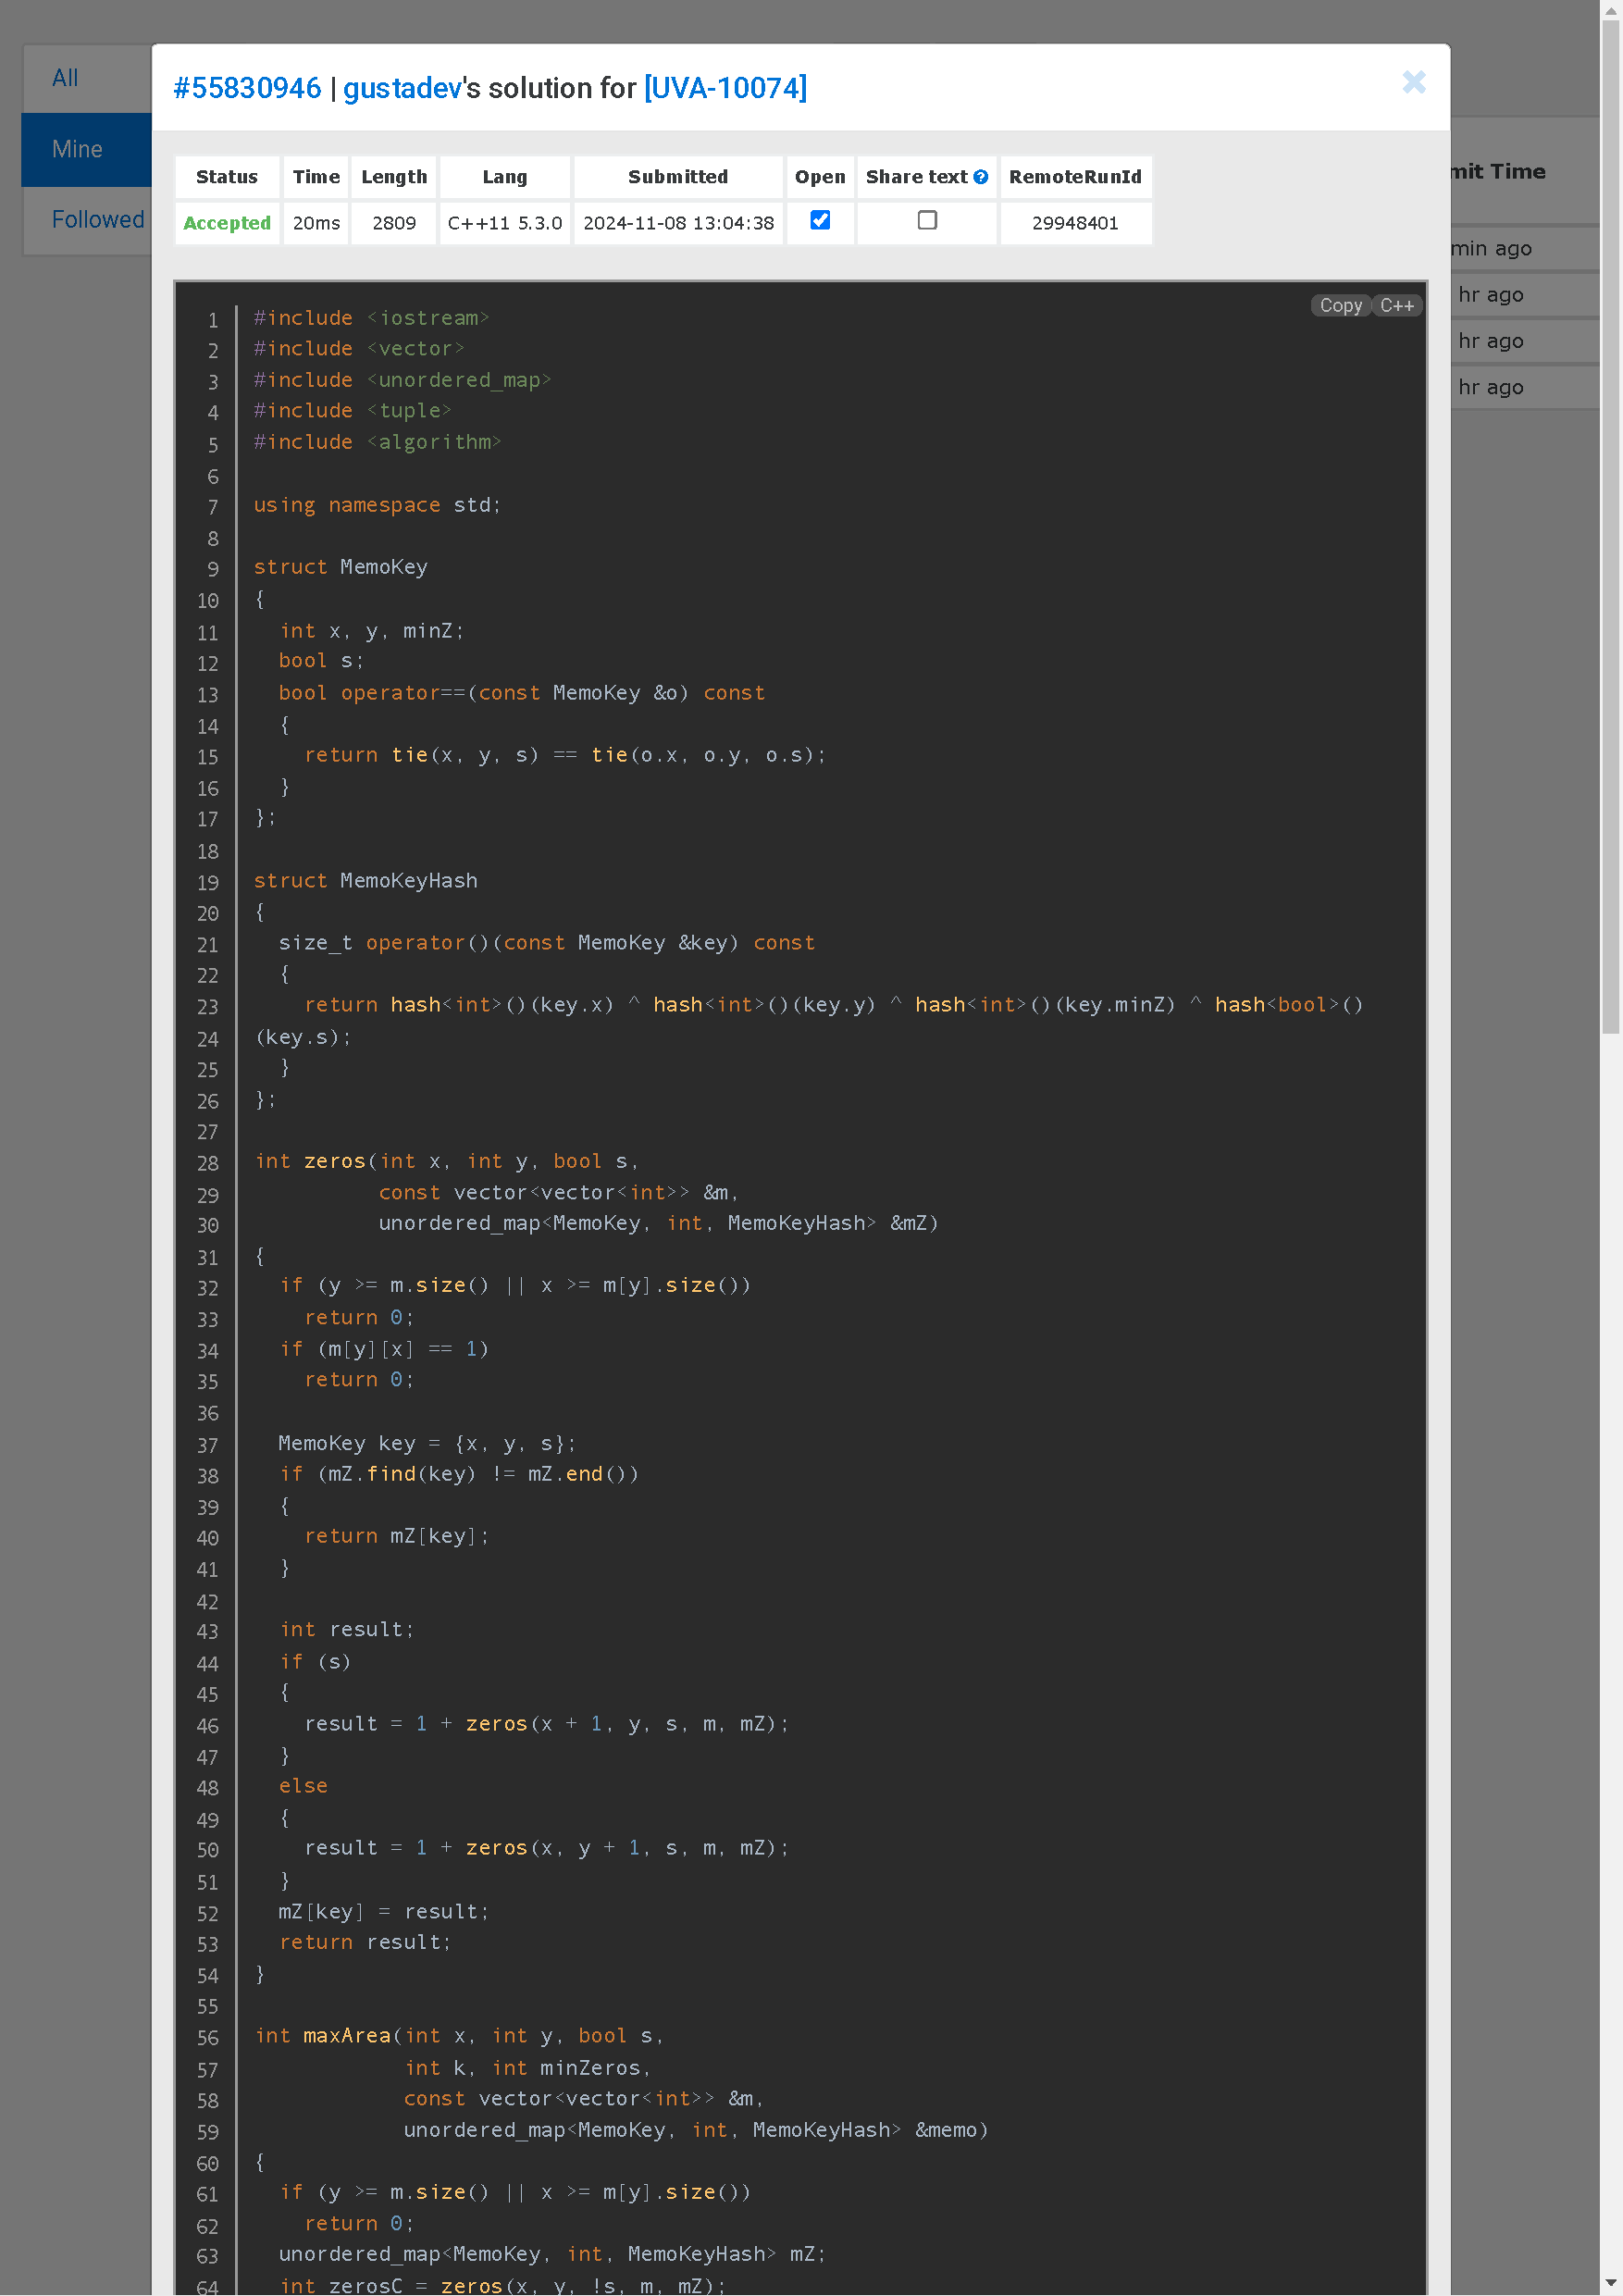
\includegraphics[clip, trim=40 0 40 25, width=17cm]{10074/submit-1.pdf}\vspace{-2cm}

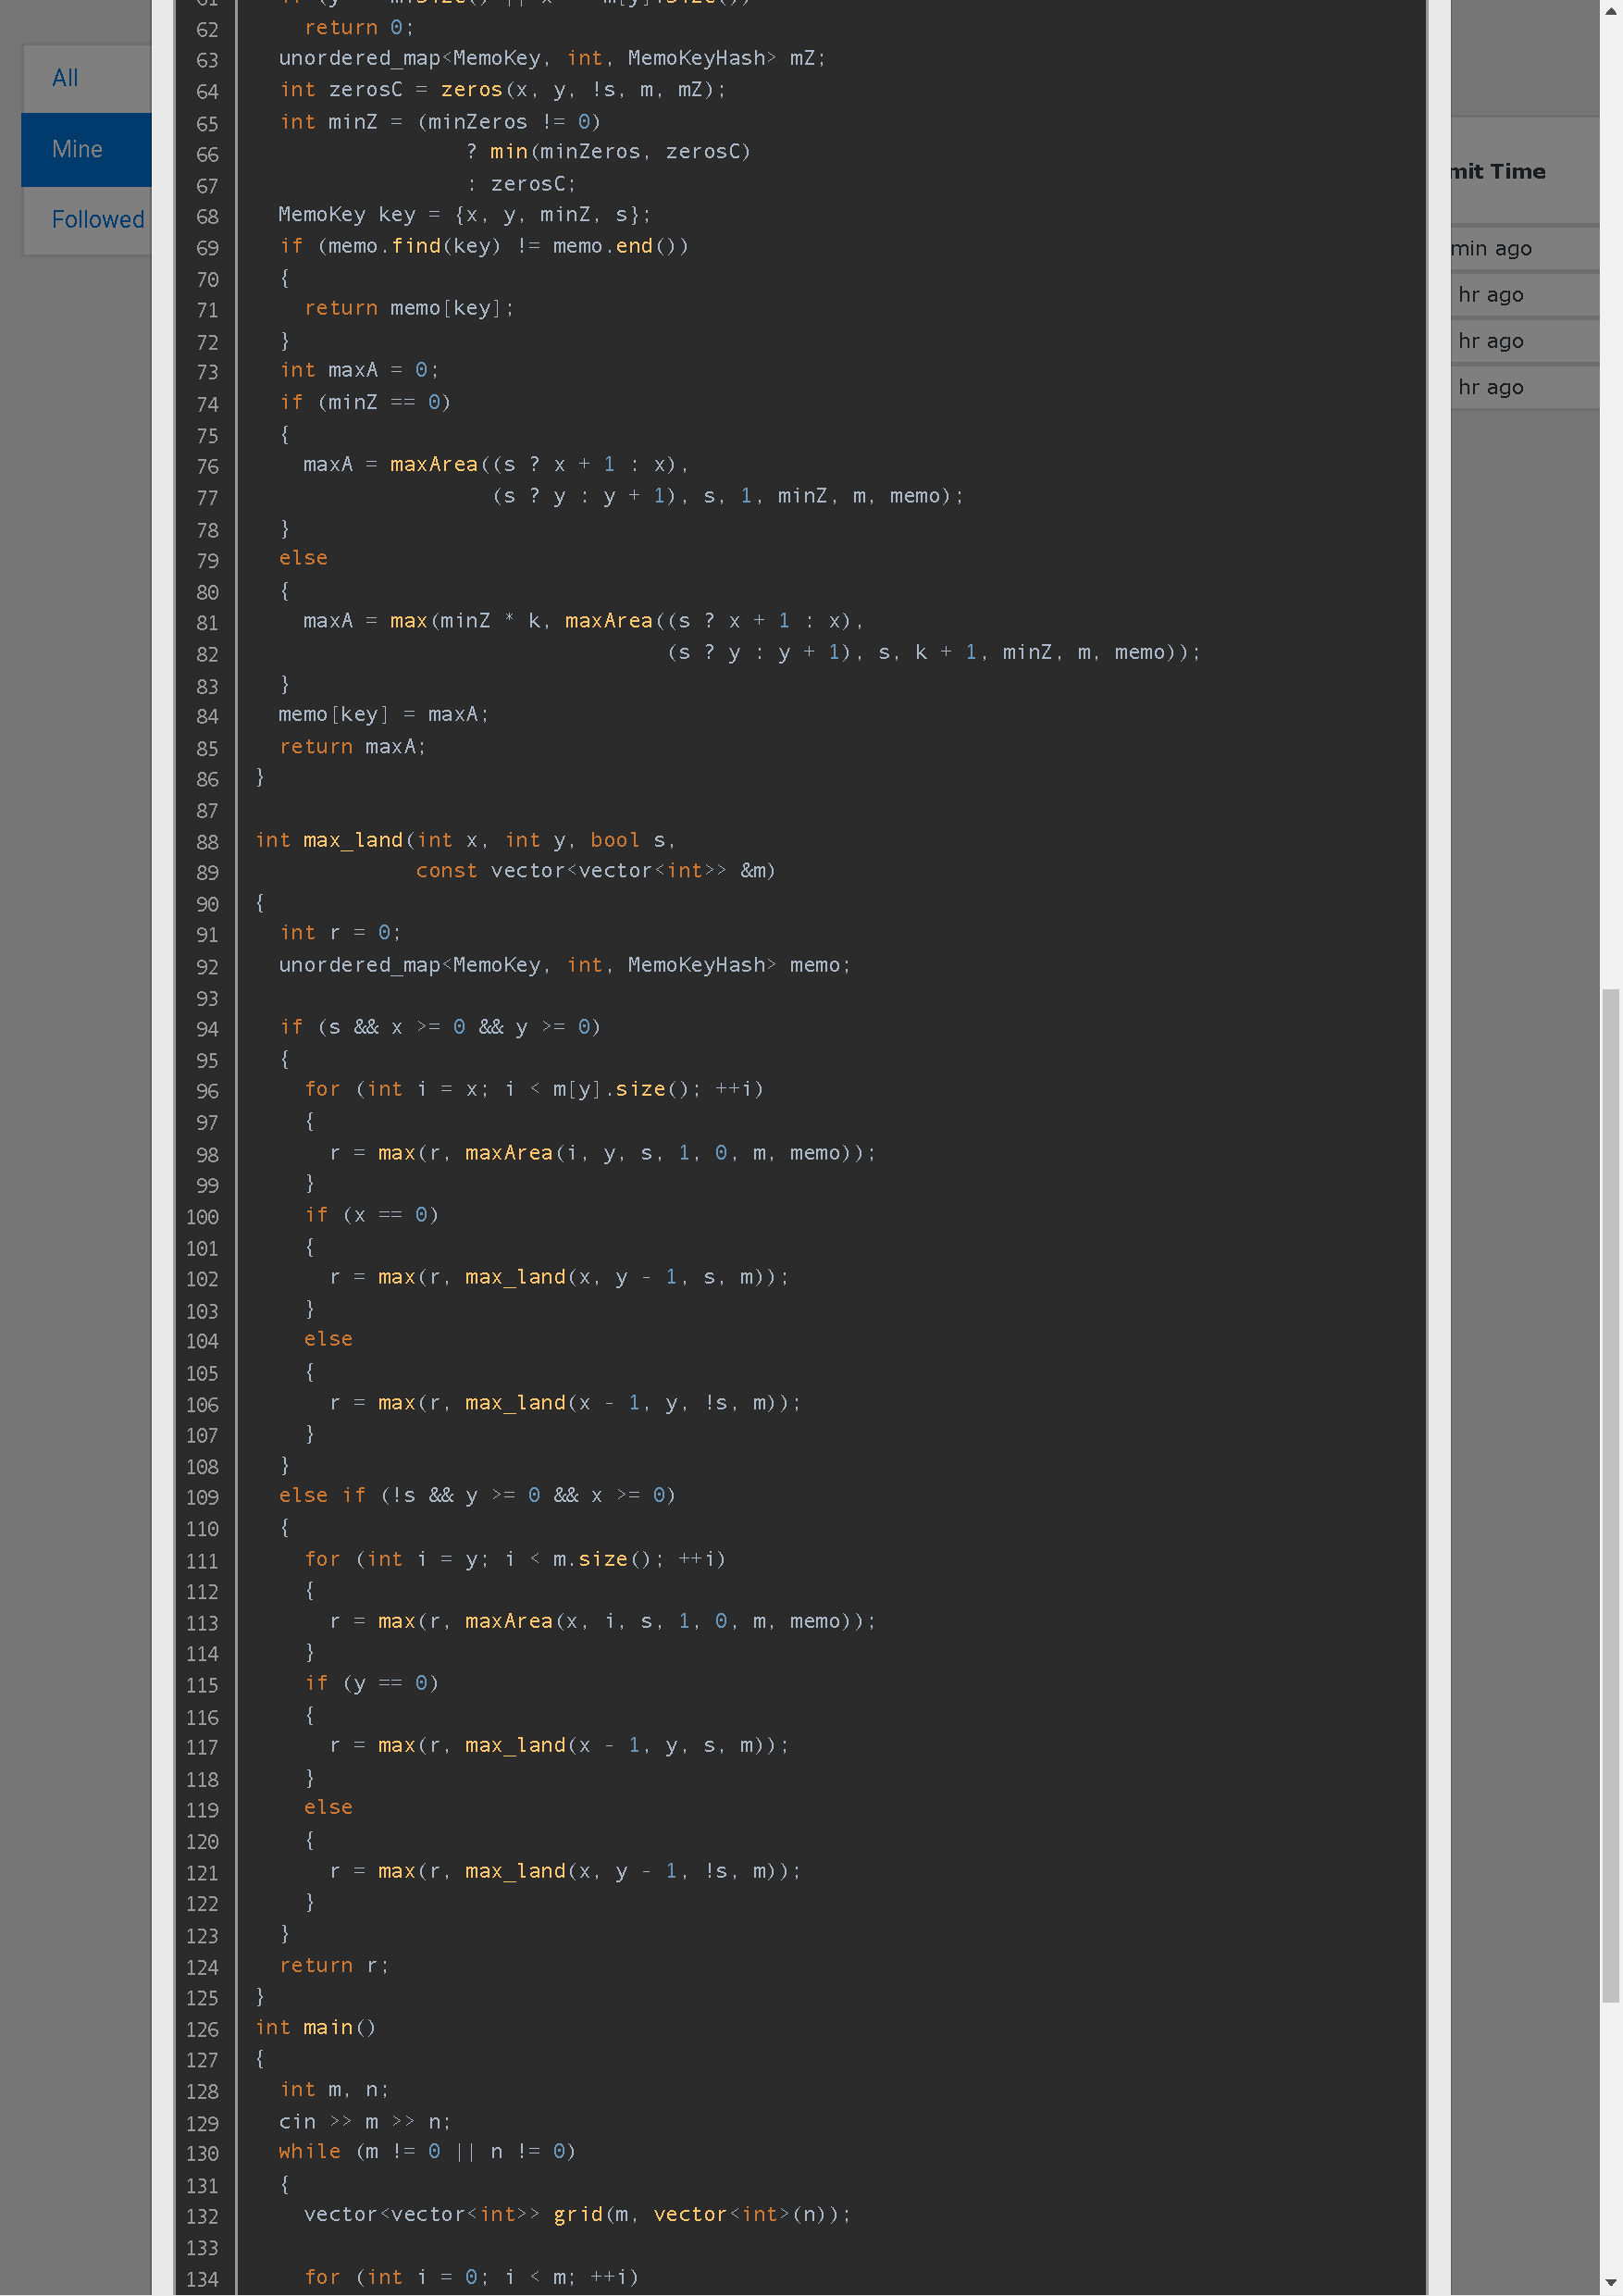
\includegraphics[clip, trim=40 0 40 25, width=17cm]{10074/submit-2.pdf}\vspace{-2cm}

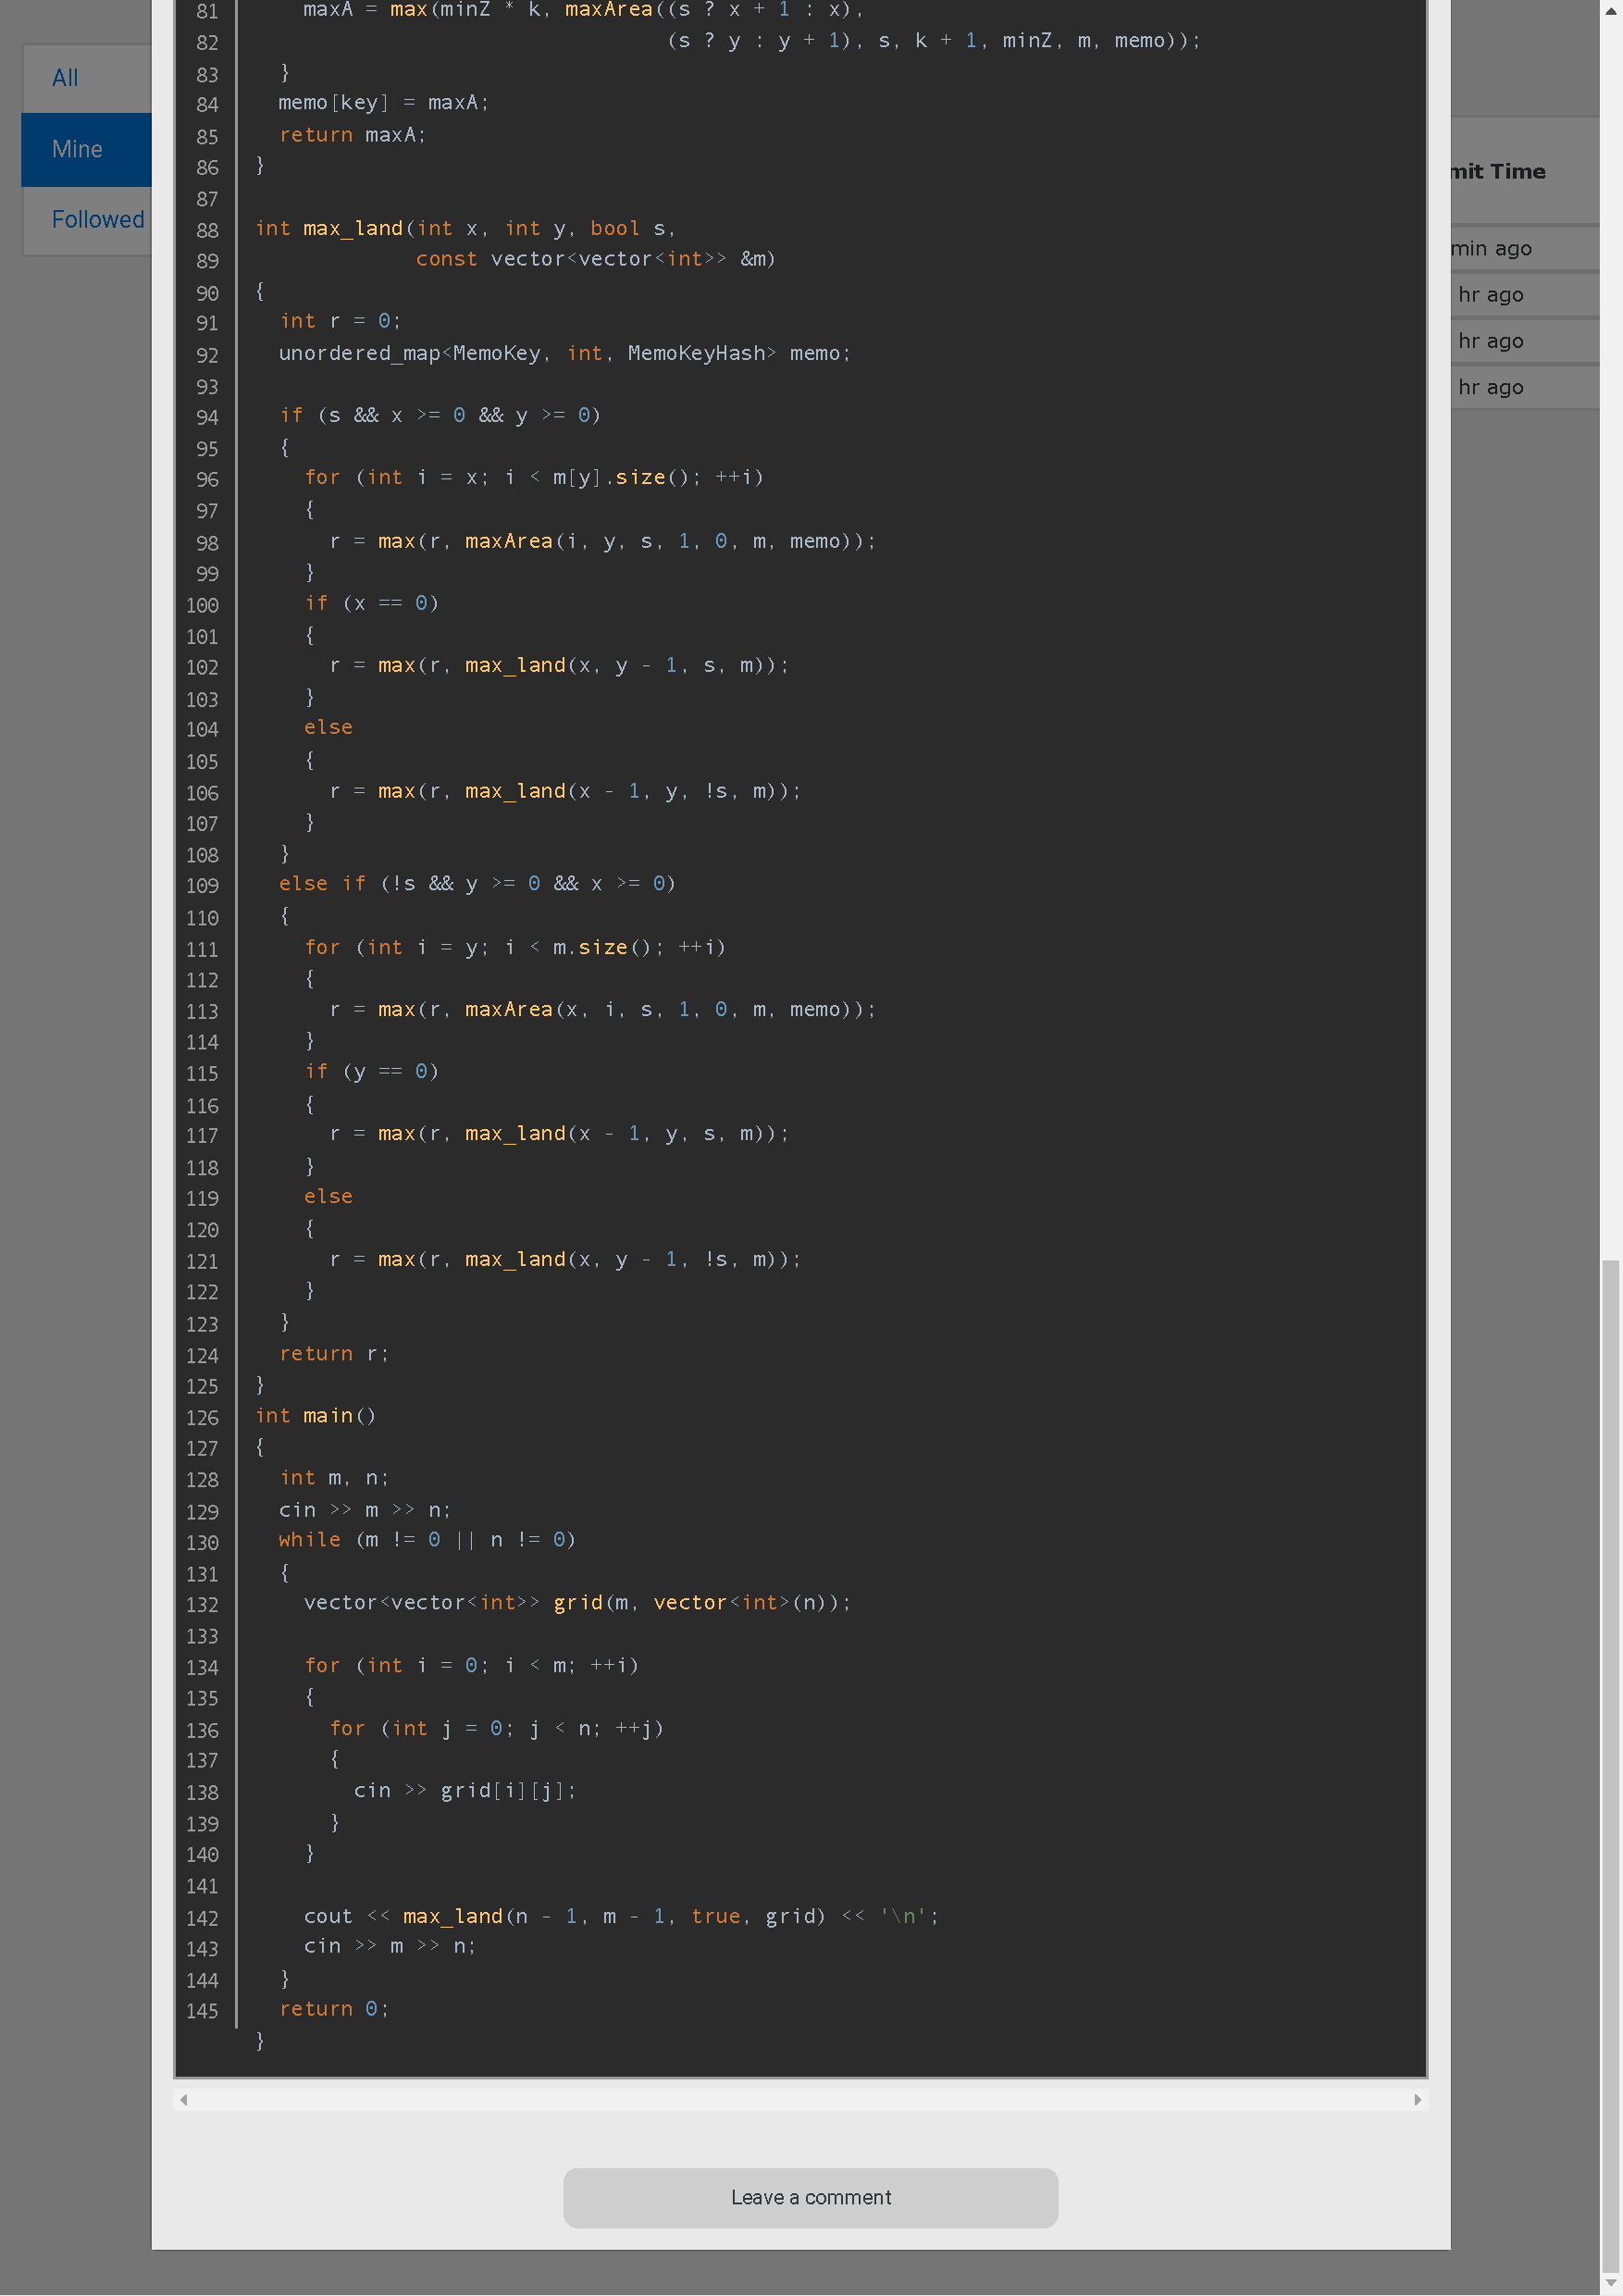
\includegraphics[clip, trim=40 0 40 25, width=17cm]{10074/submit-3.pdf}\vspace{-2cm}

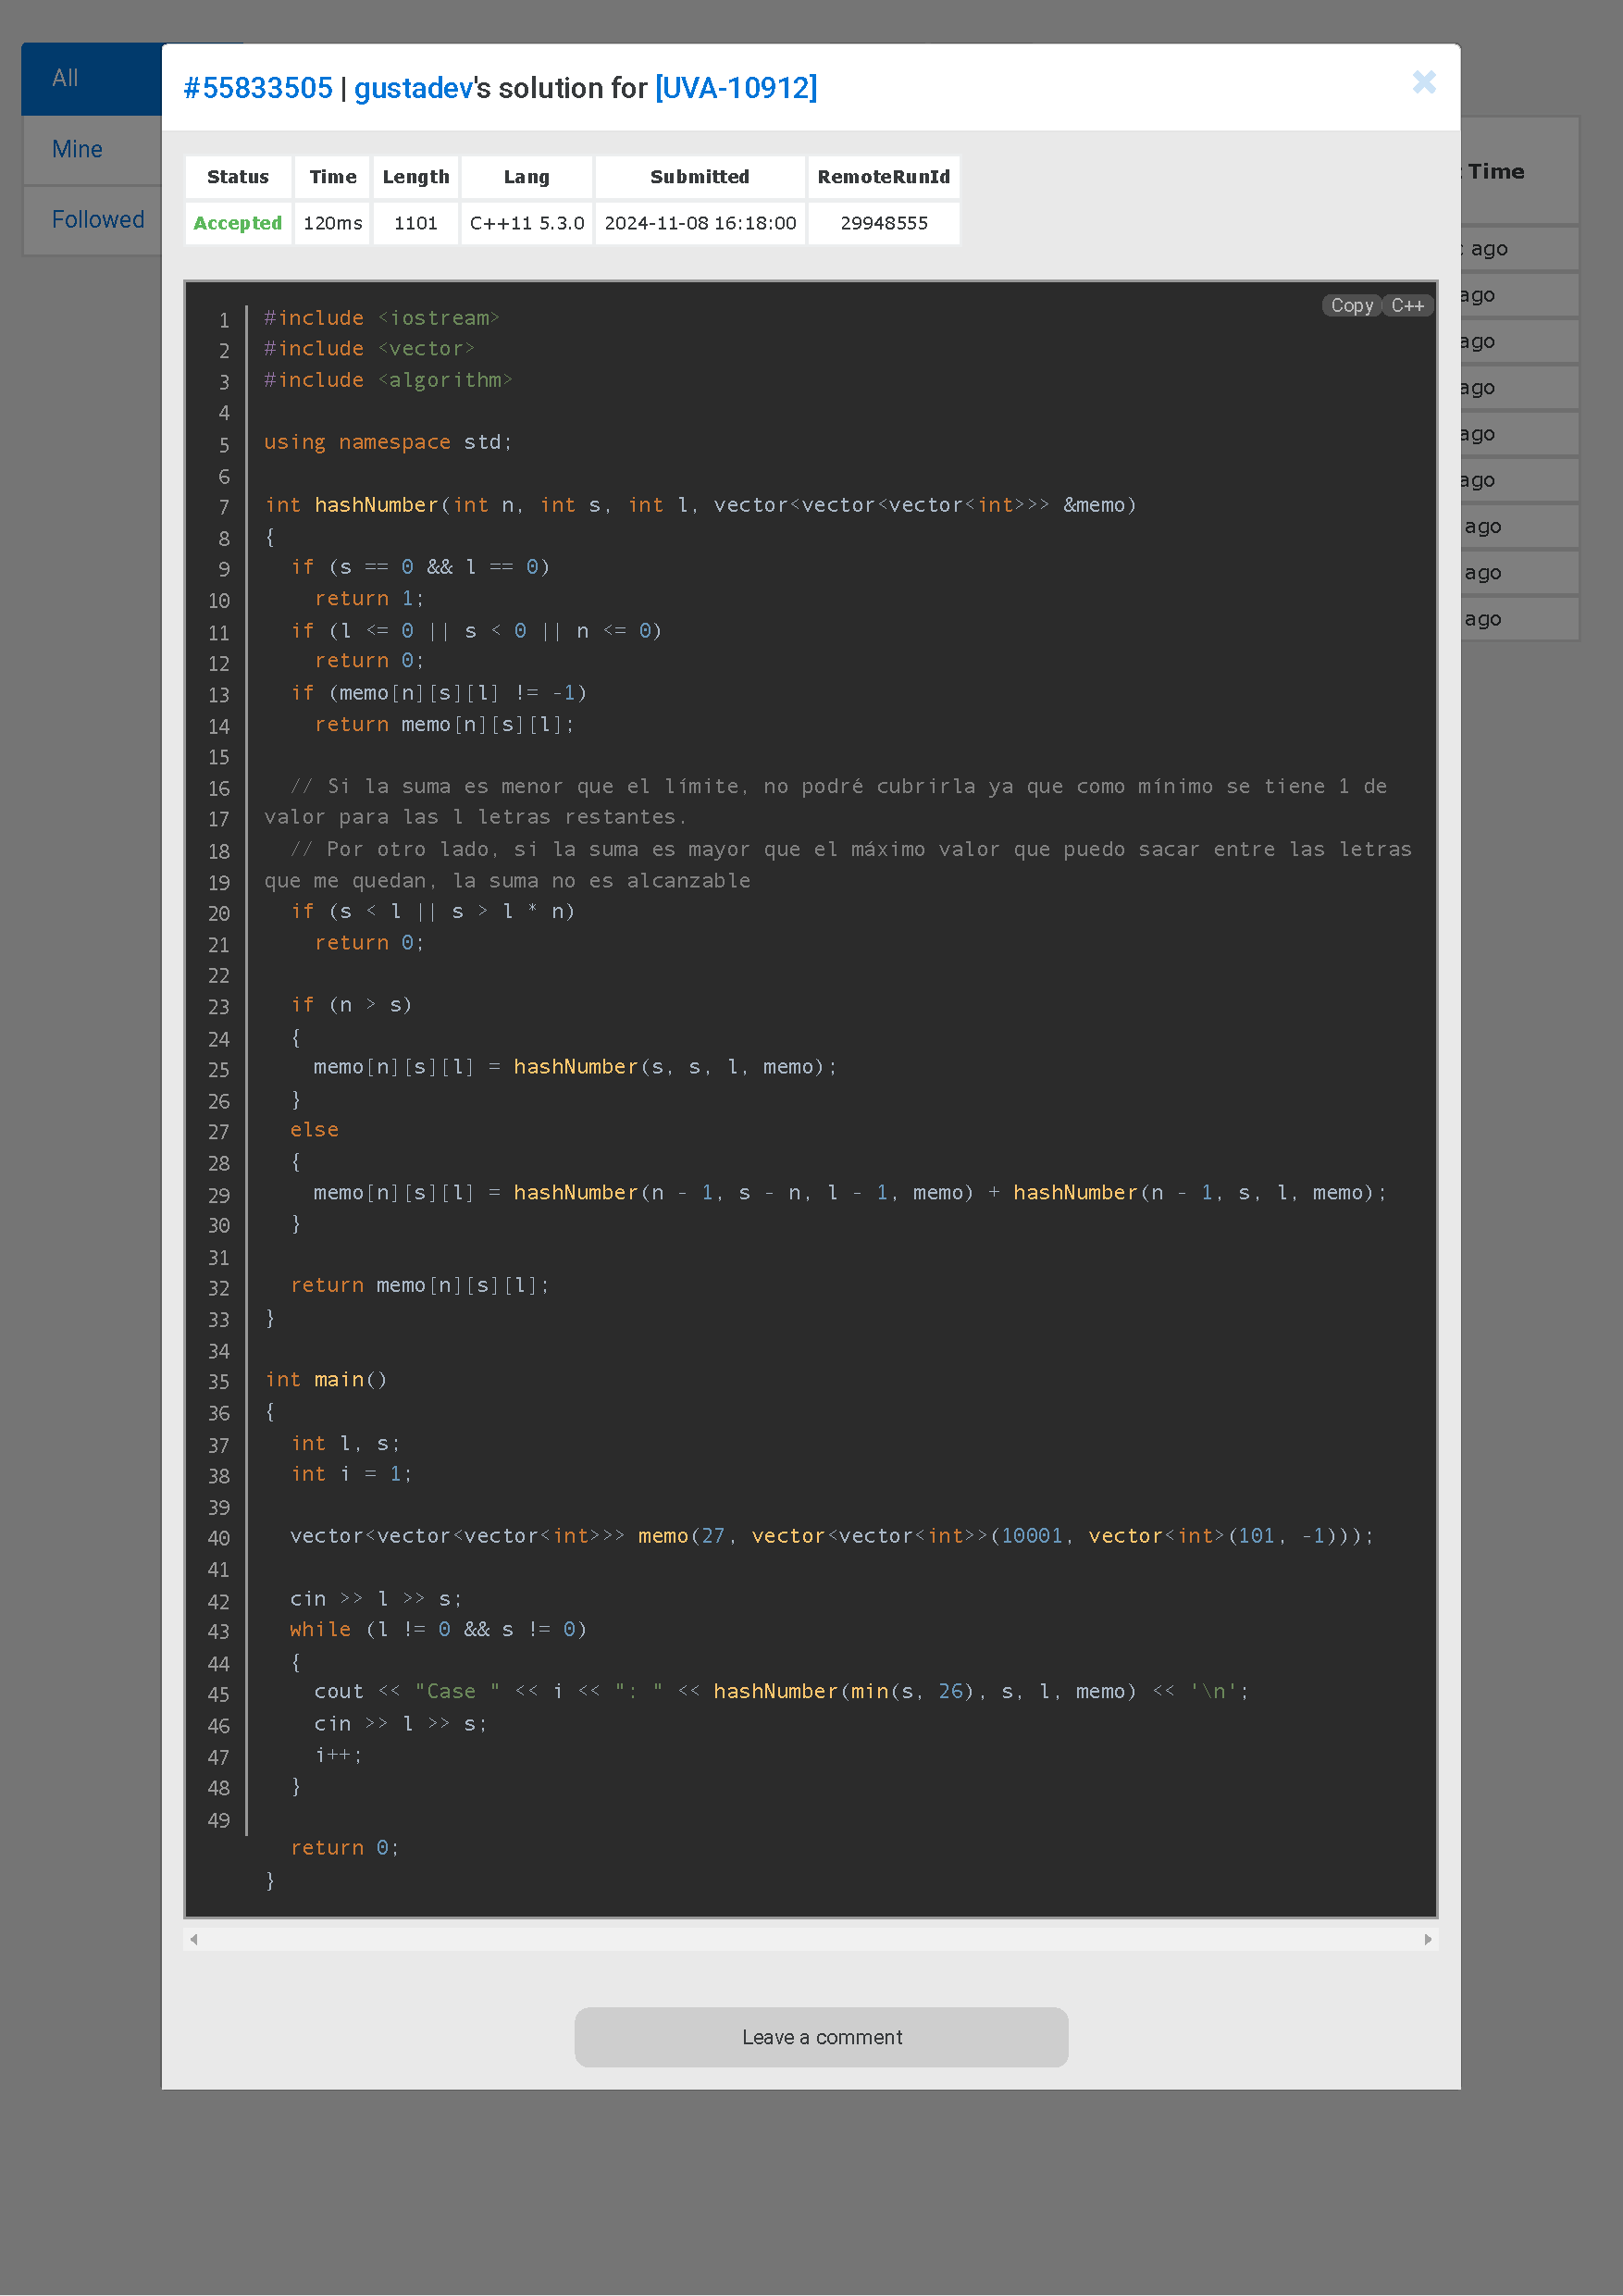
\includegraphics[clip, trim=40 0 40 25, width=17cm]{10912/submit.pdf}\vspace{-2cm}

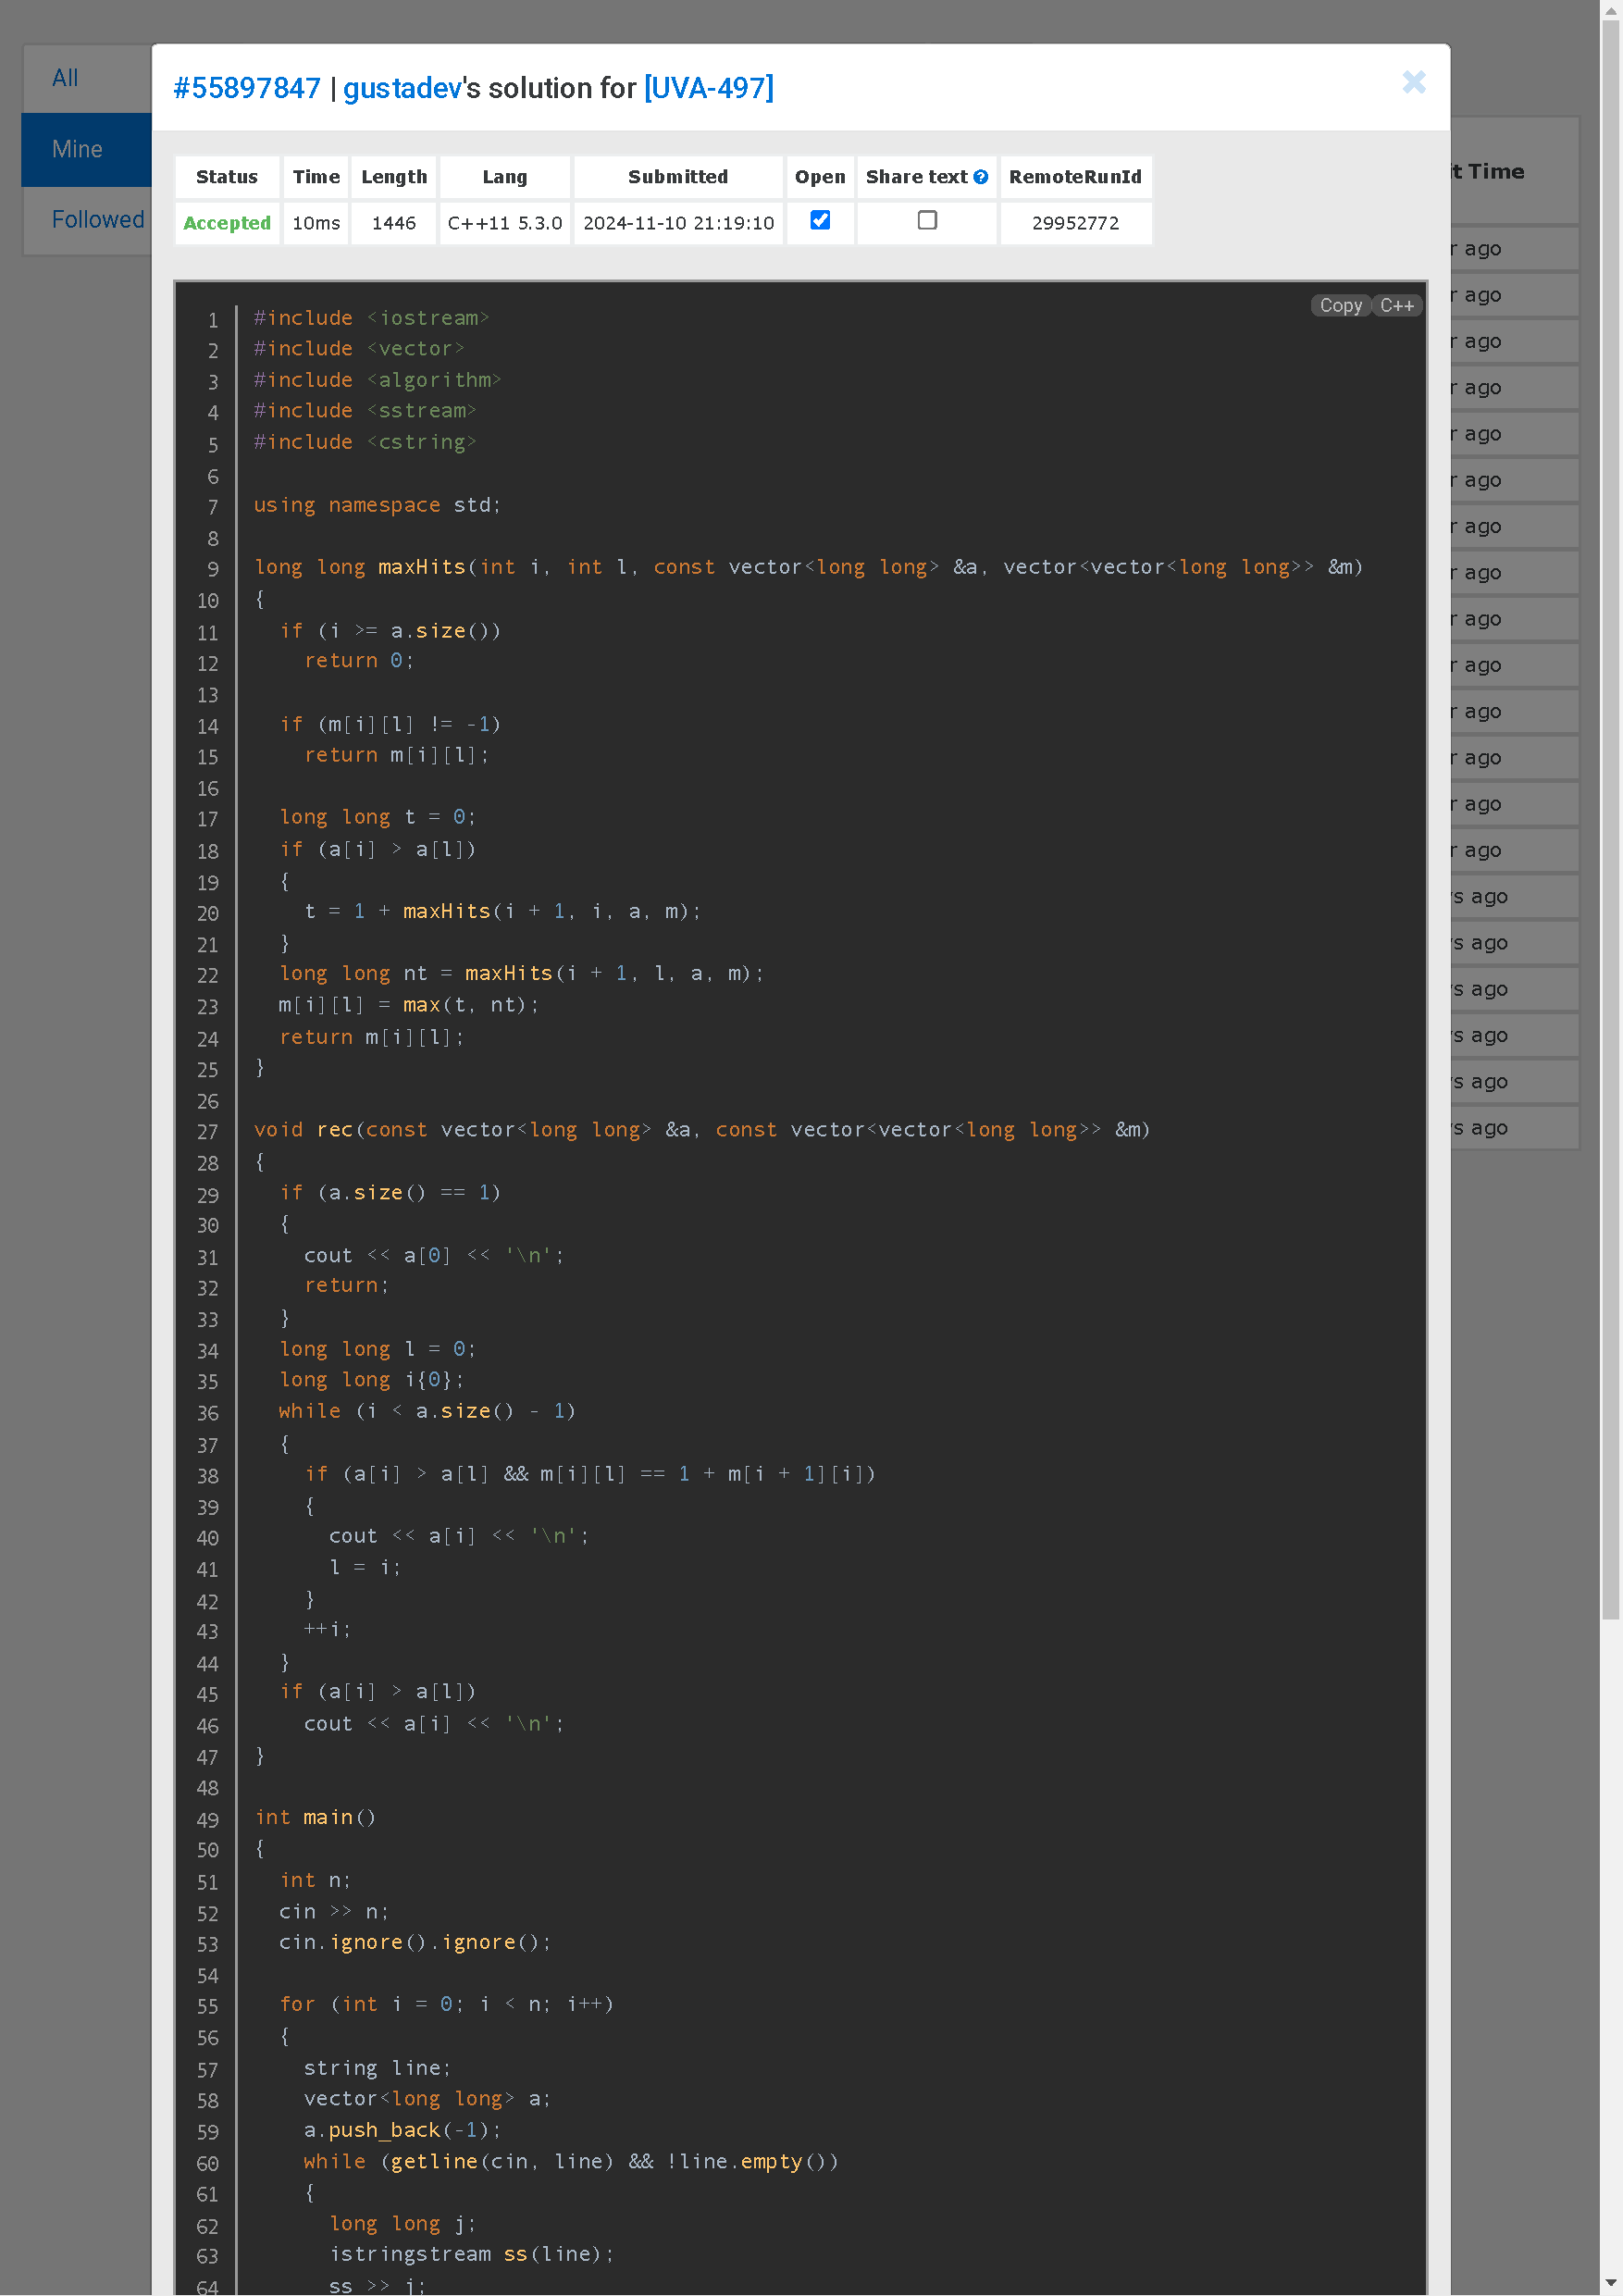
\includegraphics[clip, trim=40 0 40 25, width=17cm]{497/submit-1.pdf}\vspace{-2cm}

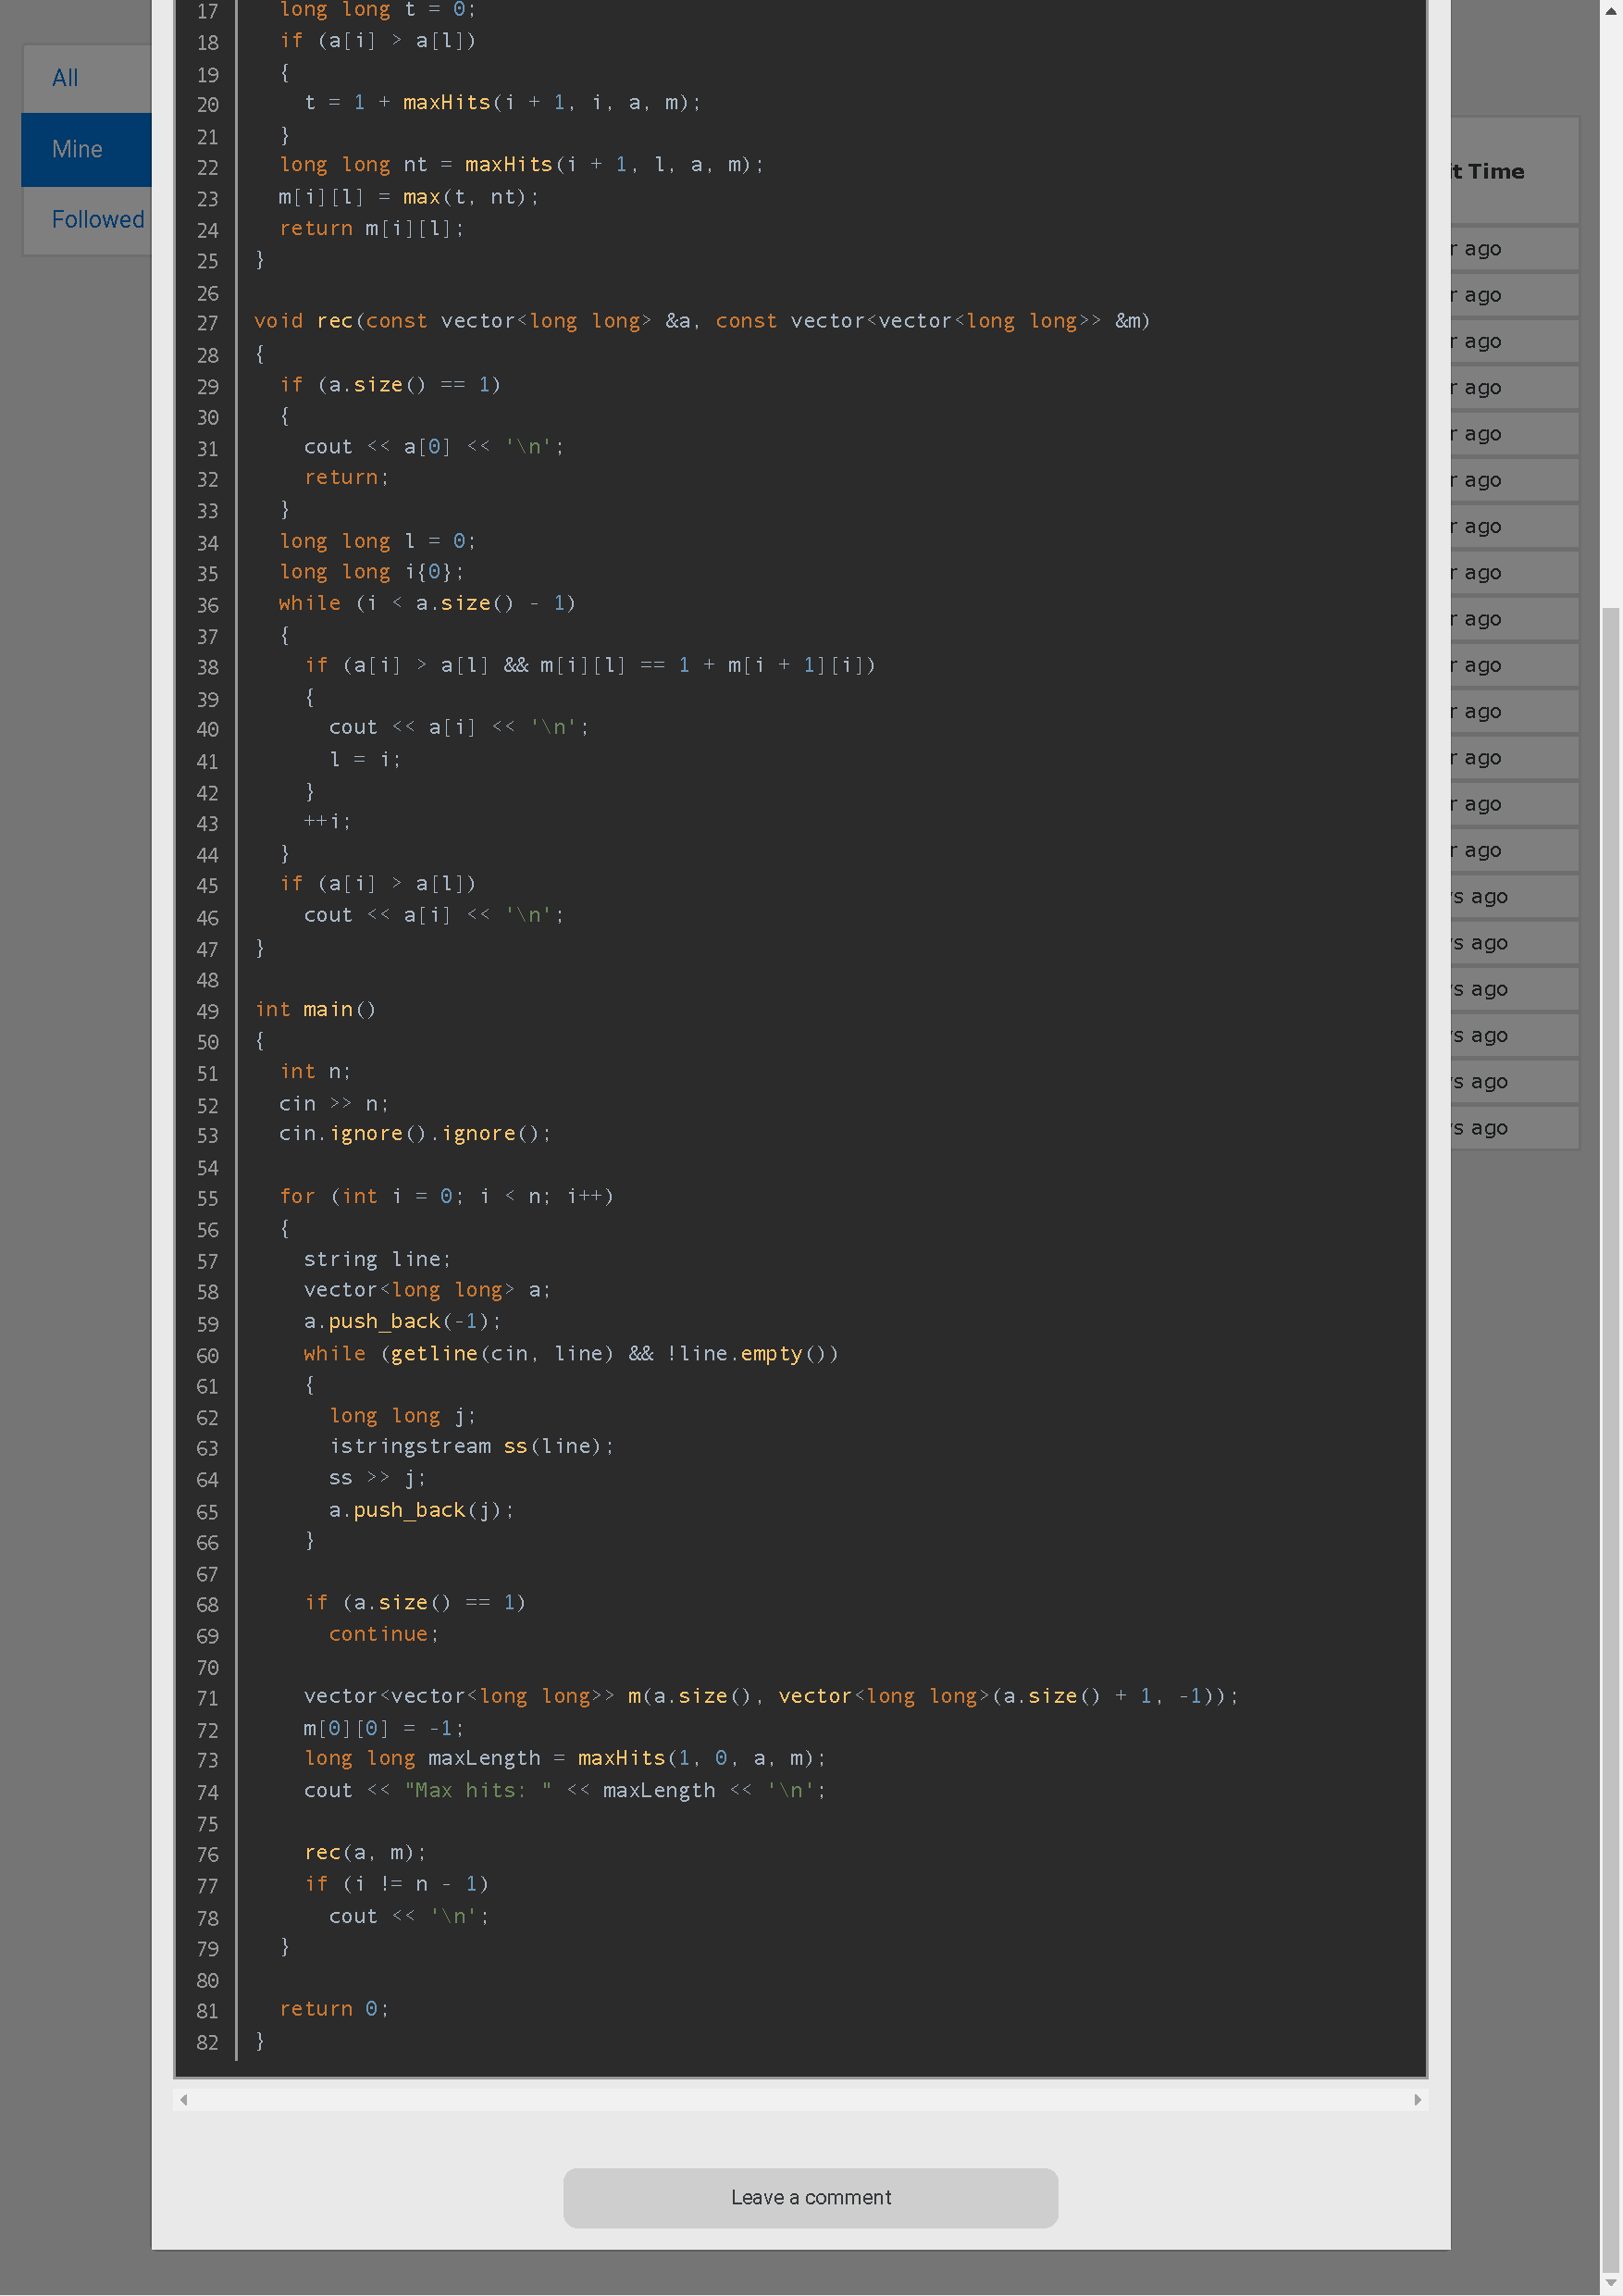
\includegraphics[clip, trim=40 0 40 25, width=17cm]{497/submit-2.pdf}\vspace{-2cm}

\end{document}
